%%%%%%%%%%%%%%%%%%%%%%%%%%%%%%%%%%%%%%%%%%%%%%%%%%%%%%%%%%%%%%%%%%%%%%
% amspaper.tex --  LaTeX-based template for submissions to American 
% Meteorological Society journals
%
% Template developed by Amy Hendrickson, 2013, TeXnology Inc., 
% amyh@texnology.com, http://www.texnology.com
% following earlier work by Brian Papa, American Meteorological Society
%
% Email questions to latex@ametsoc.org.
%
%%%%%%%%%%%%%%%%%%%%%%%%%%%%%%%%%%%%%%%%%%%%%%%%%%%%%%%%%%%%%%%%%%%%%
% PREAMBLE
%%%%%%%%%%%%%%%%%%%%%%%%%%%%%%%%%%%%%%%%%%%%%%%%%%%%%%%%%%%%%%%%%%%%%

%% Start with one of the following:
% DOUBLE-SPACED VERSION FOR SUBMISSION TO THE AMS
\documentclass{ametsoc}

% TWO-COLUMN JOURNAL PAGE LAYOUT---FOR AUTHOR USE ONLY
% \documentclass[twocol]{ametsoc}

%%%%%%%%%%%%%%%%%%%%%%%%%%%%%%%%
%%% To be entered only if twocol option is used

\journal{jcli}

\usepackage{color}
\usepackage{rotating}
\usepackage{tikz}

\DeclareDelayedFloatFlavor{sidewaysfigure}{figure}
\DeclareDelayedFloatFlavor{sidewaystable}{table}

%  Please choose a journal abbreviation to use above from the following list:
% 
%   jamc     (Journal of Applied Meteorology and Climatology)
%   jtech     (Journal of Atmospheric and Oceanic Technology)
%   jhm      (Journal of Hydrometeorology)
%   jpo     (Journal of Physical Oceanography)
%   jas      (Journal of Atmospheric Sciences)	
%   jcli      (Journal of Climate)
%   mwr      (Monthly Weather Review)
%   wcas      (Weather, Climate, and Society)
%   waf       (Weather and Forecasting)
%   bams (Bulletin of the American Meteorological Society)
%   ei    (Earth Interactions)

%%%%%%%%%%%%%%%%%%%%%%%%%%%%%%%%
%Citations should be of the form ``author year''  not ``author, year''
\bibpunct{(}{)}{;}{a}{}{,}

%%%%%%%%%%%%%%%%%%%%%%%%%%%%%%%%

%%% To be entered by author:

%% May use \\ to break lines in title:

\title{The changing character of twenty-first century precipitation over the western United States in the variable-resolution CESM}


%Future changes of precipitation over Western United States using variable-resolution CESM 

%change the title?

%%% Enter authors' names, as you see in this example:
%%% Use \correspondingauthor{} and \thanks{Current Affiliation:...}
%%% immediately following the appropriate author.
%%%
%%% Note that the \correspondingauthor{} command is NECESSARY.
%%% The \thanks{} commands are OPTIONAL.

    \authors{Xingying Huang, \correspondingauthor{Xingying Huang, 
     Department of Land, Air and Water Resources,
     University of California Davis, Davis, CA 95616.}
     Paul A. Ullrich}

     \affiliation{Department of Land, Air and Water Resources, University of California, Davis}

\email{xyhuang@ucdavis.edu}


    \extraauthor{}
    \extraaffil{}


%%%%%%%%%%%%%%%%%%%%%%%%%%%%%%%%%%%%%%%%%%%%%%%%%%%%%%%%%%%%%%%%%%%%%
% ABSTRACT
%
% Enter your Abstract here

\abstract{The changing character of precipitation frequency and intensity in the western United States over the 21st century is investigated using an ensemble of 26-year simulations with the variable-resolution Community Earth System Model (VR-CESM) at a local grid resolution of $\sim$0.25$^\circ$.  Simulations are forced using prescribed sea-surface temperatures, sea-ice extent and greenhouse gas concentrations from the representative concentration pathway (RCP) 8.5 scenario.  VR-CESM is shown to be effective at accurately capturing the spatial patterns of the historical precipitation climatology. In the Intermountain West and Southwest U.S., we observe a statistically significant increase in mean precipitation and rainy days through mid-century, although this trend is tampered by end of century in response to a decrease in relative humidity.  In the Pacific Northwest, extreme precipitation events are observed to increase significantly as a result of increased cool season integrated vapor transport.  In particular, extreme precipitation in this region appears to increase more rapidly than would be predicted by the Clausius-Clapeyron relationship.  No clear climate signal emerges in mean precipitation or for extremes in California, where the precipitation climatology is subject to large interannual variability that is tied more closely to ENSO.  Results are discussed in the context of the existing literature on precipitation extremes in the western U.S.}


\begin{document}


%% Necessary!
\maketitle


%%%%%%%%%%%%%%%%%%%%%%%%%%%%%%%%%%%%%%%%%%%%%%%%%%%%%%%%%%%%%%%%%%%%%
% MAIN BODY OF PAPER
%%%%%%%%%%%%%%%%%%%%%%%%%%%%%%%%%%%%%%%%%%%%%%%%%%%%%%%%%%%%%%%%%%%%%
%
\section{Introduction}

There is substantial and growing interest in understanding the character of precipitation within a changing climate, motivated largely by its pronounced impacts on water availability and flood management in both human and natural systems \citep{hegerl2004detectability, kharin2007changes, scoccimarro2013heavy}.  Among past studies addressing precipitation, extremes have been a major focus, particularly drought and flood events \citep{seneviratne2012changes}.  Overall, it is widely agreed that although atmospheric water vapor concentration is increasing, the impacts of a changing climate on the character of precipitation is far more complicated.  Extreme precipitation events are particularly nuanced:  Our best projections suggest that extreme precipitation events will intensify even in regions where mean precipitation decreases \citep{tebaldi2006going, kharin2007changes}.


Future climate projections, particularly those addressing the frequency and intensity of rare events, are inevitably subject to large uncertainties.  Nonetheless, climate models have been invaluable tools for developing insight into this problem \citep{easterling2000climate}. In particular, global climate models (GCMs) have often been used to investigate changes in the mean, variability and extremes of climate, as forced with predicted greenhouse gas (GHGs) concentrations and aerosol emissions \citep{meehl2006future}. Although several past studies have investigated climate extremes at the global scale \citep{seneviratne2012changes}, studies addressing extremes at local and regional scales are less common.  It is well understood how increased GHG concentrations have contributed to the observed intensification of heavy precipitation events over the tropical ocean \citep{allan2008atmospheric} and the majority of Northern Hemisphere overland areas \citep{min2011human}, but changes are much more poorly understood at regional scales where meteorological variability is large \citep{trenberth2011changes}.  As a consequence of this variability, confidence in the assessment of regional extreme precipitation changes requires both high spatial resolution and a long integration period, both of which can make the computational cost untenable for global simulations.  This issue of insufficient regional-scale climate information has been a major outstanding problem in climate science, as stakeholders and water managers typically require fine-scale information on climate impacts in order to effectively develop adaptation and mitigation strategies.


Dynamical downscaling with regional climate models (RCMs) has been one of the few tools available to ascertain the frequency, intensity, and duration of extreme events at the needed scales.  By only simulating a limited regional domain, RCMs better capture fine-scale dynamical features with high horizontal resolution \citep{bell2004regional, frei2006future, rauscher2010resolution, wehner2013very}. Higher resolution enables more accurate simulation of precipitation extremes, which are driven by circulation patterns, cloudiness, land use, land/water contrast, snowpack and topography \citep{leung2003regional, diffenbaugh2005fine, salathe2008high, wehner2010effect}. For example, \cite{leung2003hydroclimate} showed that the higher-resolution RCMs yield more realistic precipitation patterns and produce more frequent heavy precipitation over the western U.S. (WUS), consistent with observations. \cite{diffenbaugh2005fine} studied both extreme temperature and precipitation events over the contiguous United States using a RCM configured at 25 km horizontal resolution, and demonstrated that fine-scale processes were critical for accurate assessment of local- and regional-scale climate change vulnerability. \cite{salathe2008high} found significant differences in trends for temperature and precipitation over the Pacific Northwest using a high-resolution RCM for future climate simulations.  And \cite{ashfaq2016high} observed a 7.4\% increase in precipitation from extremes over the contiguous U.S. from simulations with RegCM4 driven by CMIP5 global data.


Despite their success, RCMs also have known issues associated with inconsistency between the lateral forcing data and the driven RCM.  The menu of physical parameterizations and tuning parameters typically available to RCMs can also lead to over-tuning of the model for a particular geographic region or climatological field \citep{mcdonald2003transparent, laprise2008challenging, mesinger2013limited}.  Consequently, there has been growing interest in variable-resolution enabled GCMs (VRGCMs) to improve regional climate simulations. Unlike RCMs, which require GCM data to drive the simulation at lateral boundaries, VRGCMs use a unified model with coarse global resolution and enhanced resolution over a specific study region \citep{staniforth1978variable, fox1997finite}. VRGCMs have demonstrated competitive ability for regional climate studies at a reduced computational cost, particular when compared to uniform-resolution GCMs \citep{fox2006variable, rauscher2013exploring}.


In this paper, we utilize the recently developed variable-resolution option in the Community Earth System Model (VR-CESM).  VR-CESM is based on the CESM (and its predecessor, the Community Climate System Model (CCSM)), a family of models that have been used for decades to study the global climate \citep{neale2010description, hurrell2013community}.  The overall performance of VR-CESM for modeling regional climate in the California and Nevada is detailed in \cite{huang2016evaluation}, where it was argued that VR-CESM has competitive biases in comparison to the Weather Research and Forecasting (WRF) model (a traditional RCM) and the uniform-resolution CESM, when evaluating against high-quality observations and reanalysis. VR-CESM has been used in a number of studies to simulate fine-scale atmospheric processes  \citep{zarzycki2014using, zarzycki2015effects, rhoades2015characterizing, huang2016irrigation, rhoades2016projecting}.


This study focuses on changes in the character of precipitation over the 21st century within the WUS, as predicted from long-term ensemble runs conducted with VR-CESM with a local grid resolution of $\sim$0.25$^\circ$.  The WUS is known to be particularly vulnerable to hydrological extremes, particularly floods and droughts \citep{leung2003hydroclimate, caldwell2010california}, and hosts a variety of local features and microclimates associated with its rough and varied topography.  Simulations of the future climate are performed in accordance with the representative concentration pathway (RCP) 8.5 scenario, which describes a ``business-as-usual'' projection for GHGs \citep{riahi2011rcp}.  In this study we focus singularly on the RCP 8.5 scenario because its mid-century results are similar to a more optimistic RCP2.6 scenario end-of-century.  Simulations are further conducted in accordance with the Atmospheric Model Intercomparison Project (AMIP) protocol \citep{Gates1992}, a widely-used approach for climate model diagnosis, validation and intercomparison that imposes global sea surface temperatures (SSTs) and sea ice.  It is well-known that correctly simulating changes to the spatial pattern of SSTs in state-of-the-art coupled GCMs remains a significant challenge \citep{joseph2006enso, stevenson2012significant, jha2014sst, taschetto2014cold}.  However, by constraining atmospheric boundary conditions at the sea surface, we avoid model biases that are known to exist in the fully coupled configuration \citep{grodsky2012tropical, small2014new} but accept potential uncertainties associated with our choice of SSTs.


Changes in the character of precipitation, in terms of frequency and intensity, have been assessed in our study from recent history through the end of the 21st century.  A comprehensive set of indices for precipitation extremes have been evaluated from the ensemble simulations over the 26-year periods corresponding to historical (1980-2005), mid-century (2025-2050) and end-of-century (2075-2100). Spatial inhomogeneity in local geography and temperature are observed to result in similarly inhomogeneous impacts on the precipitation field.  Teleconnections (specifically the El Nin\~o-Southern Oscillation, ENSO) are also observed to have a pronounced impact on precipitation features.  Since only one SST dataset was used for this study, we note that our projections are conditioned on a particular future character of ENSO.  This is a potentially large source of uncertainty, as at present there is no clear consensus on how ENSO may behave under a warming climate \citep{fedorov2000nino, latif2009nino, guilyardi2009understanding, collins2010impact, dinezio2012mean}, and strengthening or weakening of this pattern will have clear consequences for our results (as discussed in section \ref{sec:Results}\ref{sec:IsolatingENSO}).


This work builds on a number of previous studies that have explored the projected future change in WUS precipitation. For example, \cite{kim2005projection} applied downscaled climate change signals to selected indicators, and concluded that global warming induced by increased CO$_2$ is likely to drive increases in extreme hydrologic events in the WUS. \cite{duffy2006simulations} found that changes to mean precipitation predicted by the RCMs are not statistically significant compared to interannual variability in many regions over WUS, although there is little consistency among the different RCMs as to responses in precipitation to increased GHGs. \cite{gao2015dynamical} pointed out a potentially large increase in atmospheric river events by the end of the 21st century under the RCP8.5 scenario, with implications for large-scale and heavy precipitation events along the Pacific coast. 


This paper is structured as follows. Section \ref{sec:ModelSetup} describes the model setup.  Section \ref{sec:Methodology} describes the methodology and reference datasets employed. An assessment of the ability of the model to capture the climatology of the WUS is given in section \ref{sec:ModelAssessment} with discussions of drivers of precipitation change in section \ref{sec:ChangeDrivers}. Results from the future mean climatological trend and projected changes to precipitation indices are in section \ref{sec:Results}. Section \ref{sec:Summary} summarizes the main points of the study along with further discussion.


\section{Model Setup} \label{sec:ModelSetup}

CESM is a state-of-the-art Earth modeling framework, consisting of coupled atmosphere, ocean, land and sea ice models \citep{CAM5Tech, hurrell2013community}. In this study, the Community Atmosphere Model version 5 (CAM5) \citep{CAM5Tech} and the Community Land Model version 4.0 \citep{CLM40Tech} are used.  CAM5 is configured with the Spectral Element (SE) dynamical core, which is known for its conservation properties, accuracy and parallel scalability \citep{dennis2011cam, taylor2011conservation} and incorporates the variable-resolution option \citep{zarzycki2014using}.  CLM is employed in the \textit{unigrid} configuration, which allows the land model and atmospheric model to utilize the same model grid so eliminates the need for interpolation.  SSTs and sea ice, which are used to compute ocean-atmosphere fluxes, are prescribed in accordance with the AMIP protocol \citep{Gates1992}. The variable-resolution mesh used for this study is depicted in Figure \ref{fig:gridmesh}, in accord with our past studies \citep{rhoades2015characterizing, huang2016evaluation, huang2016irrigation, rhoades2016projecting}.


Simulations have been performed for the historical period (1979-2005, hereafter referred to as \textsf{hist}) and for two future periods: 2024-2050 (hereafter referred to as \textsf{mid}) and 2074-2100 (hereafter referred to as \textsf{end}).  Daily outputs are recorded for each period on the native SE grid and then remapped to a regional latitude-longitude mesh \citep{ullrich2015arbitrary,ullrich2016arbitrary}.  For purposes of analysis, the first year of each time period was discarded as a spin-up period to allow adequate time for the initialized land and atmosphere to equilibrate. The 26-year duration was chosen to provide an adequate sampling of annual variability for each time phase. As mentioned earlier, GHG concentrations are set based on RCP8.5. Historical SSTs and sea ice are prescribed at 1$^\circ$ resolution, as described by \citet{hurrell2008new}. SSTs and sea ice for each future period are developed from fully-coupled RCP 8.5 climate simulations from CESM with bias correction applied  (Cecile Hannay, personal communication).  Annually-updated land surface datasets, which prescribe land-use characteristics, are interpolated from $0.5^\circ$ to the land model grid.


Ensemble runs are needed to ensure that the sample adequately accounts for climate variability, especially for statistics associated with climatological extremes. However, the exact number of ensemble members required is heavily dependent on the variability of the particular metric being examined, and so no standard ensemble criteria exists. \cite{deser2012uncertainty} suggest that around 3 ensemble runs are required to detect a significant epoch difference for JJA (June-July-August) surface temperatures, whereas 10 to 30 ensemble members are needed for that for DJF (Dec.-Jan.-Feb.) precipitation. In our study, the use of prescribed SSTs does reduce the intrinsic variability of the climate system (see supplement Figure S1-S3), and so we found reasonably converged results with two ensemble members for the historical period and four ensemble members for each future period.


\section{Methodology} \label{sec:Methodology}

\subsection{Precipitation indices}

Standard indices have been employed to characterize precipitation \citep{tebaldi2006going, zhang2011indices, sillmann2013climate}. In order to choose a comprehensive (but minimal) set that are informative to stakeholders and water resource managers, indices from throughout the literature were compiled.  The indices examined include those defined by the Expert Team on Climate Change Detection and Indices (ETCCDI) \citep{karl1999clivar} that are featured in earlier studies \citep{duliere2011extreme, sillmann2013climate, diffenbaugh2005fine, singh2013precipitation} and others such as return levels, dry spell and wet spell characteristics defined by either percentiles or by selected thresholds. As a result, the indices we have chosen for this study attempt to provide a relatively comprehensive characterization of precipitation, and are summarized in Table \ref{tab:table1}. Indices related to dry spells of variable duration have been investigated in this study, but only exhibited significant differences for extremely short ($\leq$ 5 days) dry spells and so are not included in our results.


\subsection{Impacts of ENSO}

The impact of ENSO on precipitation is emphasized in our study due to its influence on precipitation over a majority of our study area, particularly the southwest U.S. \citep{cayan1999enso, zhang2010influence, deser2012communication, yoon2015increasing}. The phase of ENSO (\textit{i.e.} El Ni\~no and La Ni\~na) is identified each year using the Oceanic Ni\~no Index (ONI), defined as the 3-month running means of SST anomalies in the Ni\~no 3.4 region (covering 5N-5S, 120-170W based on \cite{noaaElNino}). An El Ni\~no or La Ni\~na episode is said to occur when the ONI exceeds +0.5 or -0.5 for at least five consecutive months for a water year (i.e. from July to June) \citep{noaaElNino} (see the supplement Figure S6). In order to adjust for the trend in the SST field associated with climate change, the anomaly is computed against the detrended mean SSTs from the periods 2020-2050 and 2070-2100 for \textsf{mid} and \textsf{end} respectively, using the aforementioned predicted SST dataset. As argued by \cite{kao2009contrasting}, it may be desirable to use an extended Ni\~no 3.4 region to determine the phase of ENSO -- however, when employing SST anomalies integrated over a extended region 105-170W, we observed no significant impact on ONI statistics.


\subsection{Assessing statistical significance}

Student's t-test has been used to determine whether or not two datasets at each grid point are statistically equivalent, if the sample population can be adequately described by a normal distribution. The normality of a dataset is assessed under the Anderson-Darling test. When the sample populations do not approximately follow a normal distribution, Mann-Whitney-Wilcoxon (MWW) test is employed in lieu of the t-test. All tests are evaluated at the 0.05 ($\alpha$) significance level. When comparing different time periods, statistical tests are conducted by treating all years from all ensemble members as independent samples ($26 \times 2$ sample years for \textsf{hist} and $26 \times 4$ sample years for \textsf{mid} and \textsf{end}).


\subsection{Reference datasets}

Gridded observational datasets and reanalysis of the highest available quality, with comparable horizontal resolutions to our VR-CESM simulations, are used for assessing the simulation quality. Multiple reference datasets are necessary due to the underlying uncertainty in the precipitation field. The three datasets employed are as follows:

\begin{itemize}
\item[] \textbf{UW Gridded Data:}  The 0.125$^\circ$ UW daily gridded meteorological data is obtained from the Surface Water Modeling group at the University of Washington, covering the period 1949-2010 \citep{maurer2002long, hamlet2005production}. The UW dataset imposes topographic corrections by forcing the long-term average precipitation to match that of the Parameter-elevation Regressions on Independent Slopes Model (PRISM) dataset.

\item[] \textbf{National Centers for Environmental Prediction (NCEP) Climate Prediction Center (CPC):}  The 0.25$^\circ$ CPC daily dataset provides gauge-based analysis of daily precipitation covering the period 1948-2006. It is a unified precipitation product that covers the Conterminous United States and amalgamates a number of data sources at CPC via optimal interpolation objective analysis.

\item[] \textbf{North American Regional Reanalysis (NARR):}  The $\sim$32 km NCEP NARR reanalysis provides 3-hourly precipitation snapshots, obtained by dynamical downscaling over North America and covering the period 1979-present \citep{mesinger2006north}.
\end{itemize}



\section{Assessment of Precipitation Character in VR-CESM} \label{sec:ModelAssessment}

Before proceeding, we assess the ability of VR-CESM to represent the character of precipitation over the WUS.  The indices defined in Table \ref{tab:table1} are depicted in Figures \ref{fig:histEval1}, \ref{fig:histEval2} and \ref{fig:histEval3} for VR-CESM and each of the reference datasets over the historical period (1980-2005).  We assume equal confidence in each of the reference datasets, and use Student's t-test (with UW, CPC and NARR as the three statistical samples) to identify regions where VR-CESM deviates significantly from the reference mean.  Regions where differences are statistically significant in the VR-CESM dataset are identified with stippling.


Overall, VR-CESM accurately captures the spatial patterns of precipitation (spatial correlation coefficients larger than 0.9 as compared to the observations) and its indices.  As expected, the majority of precipitation is distributed along the northwest coast and the mountainous regions of the Cascades and the Sierra Nevada.  Nonetheless, several apparent biases are present:

First, VR-CESM significantly overestimates Pr over dry regions with differences between 0.2 mm to 1.5 mm, and over the eastern flank of the Cascades and on both sides of the Sierra Nevada (with relative differences reaching 50$\%$-150$\%$).  As with many regional models, VR-CESM is ``dreary'' and exhibits too many precipitation days (R1mm, Pr$\geq$1 mm/day and R5mm, 1 mm/day$\leq$ Pr $\leq$ 5 mm/day) (see Figure \ref{fig:histEval1} and \ref{fig:histEval2}) \citep{stephens2010dreary}. The spatial correlations are about 0.85, 0.75, 0.8 and 0.9 for R1mm, R5mm, R10mm and R20mm compared to the references. Nonetheless, over most regions the relative contribution of each precipitation frequency subset to total precipitation (F1mm, F5mm, F10mm, F40mm) is moderately represented by the model (with spatial correlations ranging between 0.7 to 0.8), suggesting a properly representation of the overall frequency distribution for the precipitation intensity.

Second, the spatial pattern of precipitation intensity (SDII) matches well between VR-CESM and references (spatial correlations around 0.85) with agreement everywhere except in the Great Plains (the eastern edge of our domain) and in California's Central Valley.  The Great Plains is not a focus of this study, but the suppressed intensity is primarily during the warm season (April-September) and so likely represents a failure of the convection scheme to adequately simulate variability in this region.  This bias is also observed in 0.25$^\circ$ uniform-resolution CESM simulations \citep{small2014new}, and so is not a symptom of the eastern edge of the variable-resolution transition region.

However, the grossly exaggerated intensity over the western flank of the Sierra Nevada through California's Central Valley does merit some additional discussion. Here, the overestimation of precipitation and enhanced intensity is associated with too many extreme precipitation events (Pr$>$20 mm/day) (see Figure \ref{fig:histEval3}, R40mm and Rxmm).  This bias is related to exaggerated orographic uplift (upslope winds) and triggers a dry bias along the eastern flank of the Sierras.  Similar biases in simulating extreme precipitation over topographically complex regions have also been found in high-resolution RCM smulations, and have been primarily attributed to excessively strong winds \citep{walker2009evaluation, singh2013precipitation}.  This issue may be further impacted by the diagnostic treatment of precipitation in CAM5 \citep{morrison2008new, gettelman2008new}.

The representation of precipitation in VR-CESM over California was also discussed in \cite{huang2016evaluation}, where it was observed that VR-CESM simulations at 0.25$^\circ$ adequately represented regional climatological patterns with high spatial correlation. VR-CESM demonstrated comparable performance to WRF at 27 km (which was forced with ERA-Interim reanalysis), but still overestimated overall winter precipitation compared to reference datasets (by about 25$\%$-35$\%$), with the largest differences over the western edge of the Sierra Nevada.  This bias is not alleviated by simply increasing the spatial resolution, as experimental VR-CESM simulations at 14km, 7km and 3.5km show only modest improvement (Alan M. Rhoades, personal communication).  This suggests that the bias might be related with more complex dynamic processes rather than treatment of the orographic effects. 


CESM at $\sim$1$^\circ$ resolution was also assessed in order to better understand the impacts of resolution. Overall, we find that precipitation patterns over complex topography are poorly represented in the 1$^\circ$ dataset without capturing the spatial patterns induced by orographic effects (see Figure \ref{fig:resEffect}).  Over the Cascades and Sierra Nevada, total precipitation is grossly underestimated by the 1$^\circ$ data compared to gridded and reanalysis datasets. Precipitation has otherwise been smoothed out over the coastal areas and the mountainous regions of the northwest U.S when simulated with CESM at coarse resolution.  This result clearly underscores the benefits of high resolution (particularly the representation of topography) in simulating precipitation features.  Results are also provided in the supplement for the output from a globally-uniform CESM run at 0.25$^\circ$ spatial resolution with the finite volume (FV) dynamical core \citep{wehner2014effect}, which exhibits similar performance to VR-CESM (also see the supplement Figure S3 {\color{red}to add}).  Overall, 0.25$^\circ$ resolution appears to provide the best tradeoff between accuracy and computational cost, as coarser resolution does not correctly represent precipitation features and higher resolution does not appear to substantially improve model accuracy (at least in this version of CAM).


We have also assessed the impact of the ENSO signal within the historical VR-CESM runs by differencing the precipitation fields between the warm phase (i.e. El Ni\~no) and cool phase (i.e. La Ni\~na), compared to references (see the supplement Figure S5). ENSO exhibits a weaker signal for observational precipitation, compared to VR-CESM, which might suggest that the model exaggerates ENSO's impact on precipitation, especially over the northwest U.S. The improvement of ENSO in the model is directly proportional to the representation of ENSO-forced precipitation anomalies \citep{achutarao2006enso}.



\section{Drivers of Climatological Precipitation Change} \label{sec:ChangeDrivers}

The remainder of this paper now focuses on model predictions of precipitation change over the 21st century.  Precipitation has been observed and modeled to be modified in character at both global and regional scales under climate change. The observed intensification of heavy precipitation events over the the recent past for the majority of Northern Hemisphere land areas is primarily attributed to increases in GHGs \citep{min2011human}.  GHGs drive radiative changes in the lower troposphere, increase SSTs and lead to increased evaporation, all of which then impact the character of precipitation events \citep{allen2002constraints, sugi2004mechanism}. Several studies have argued that precipitation extremes will intensify continuously through the end of 21st century in both dry and wet regions, although the extent of this change will be spatially heterogeneous \citep{donat2016more}.


In accordance with the Clausius-Clapeyron (C-C) relationship, saturation vapor pressure in the atmosphere is expected to increase by $\sim$7$\%$ for each 1$^\circ$C increase in temperature \citep{allan2008atmospheric}.  As long as a source of water vapor is present, a corresponding increase in atmospheric water vapor content is expected.  Naturally, evaporation over the ocean will intensify with climate warming, but increases in water vapor content over land may be constrained by soil moisture \citep{cayan2010future}. When specific humidity is high, heavy rain events become more probable, even if total precipitation is decreasing \citep{allen2002constraints, trenberth2011changes}.  This suggests that global total precipitation is expected to increase at a slower rate than precipitation extremes \citep{allan2008atmospheric}. In accordance with previous studies (e.g. \cite{allan2008atmospheric, o2009physical, min2011human}), changes to extreme precipitation follow the C-C relationship more closely than total precipitation amount \citep{trenberth2003changing}. However, there is still substantial uncertainty regarding the magnitude of this change, since precipitation extremes are also dependent on factors such as the vertical velocity profile and temperature \citep{o2009physical}.

With overland water vapor constrained by soil moisture content, changes to moderate or heavy precipitation events over the WUS are mainly the result of increased large-scale vapor transport from the eastern Pacific Ocean rather than directly from evaporation, typically associated with atmospheric rivers (ARs) and/or orographic uplift \citep{trenberth2003changing, neiman2008meteorological}. Warming may lead to enhancement of the storm track, which would increase ARs along the U.S. west coast with increased air water vapor content in the future \citep{dettinger2011climate, gao2015dynamical}.


The precipitation of the WUS has strong inter-annual variability caused by large-scale atmospheric circulation mainly associated with the ENSO \citep{leung2003hydroclimate}. As a significant driver of precipitation, ENSO modulates the storm track behavior over western U.S. with a northwest/southwest precipitation dipole \citep{gershunov1998interdecadal}, as discussed in \ref{sec:Results}\ref{sec:IsolatingENSO}. The projected SSTs used in this study emerge from one possible realization of ENSO. However, there is still substantial uncertainty regarding how El Ni\~no will change under global warming \citep{fedorov2000nino, guilyardi2009understanding}, which is a source of uncertainty in our results. \cite{capotondi2013enso} showed that the diversity of El Ni\~no characteristics in CCSM4 is comparable to what was found in observations, although, as found by \cite{deser2012enso}, the overall magnitude of ENSO in CCSM4 is overestimated by $\sim$30$\%$ over the preindustrial time period.


\section{Results} \label{sec:Results}

\subsection{Mean climatology} \label{sec:ResultsMeanClimatology}

Differences in the mean climate of the WUS, as predicted by VR-CESM across time periods, are depicted in Figure \ref{fig:meanClm}. Since the character of WUS precipitation has a strong seasonal contrast, changes to mean precipitation, near-surface temperature and near-surface relative humidity are depicted for what we refer to as the cool season (October to March) and the warm season (April to September).

As a result of enhanced GHG concentrations, mean annual near-surface temperature (Tavg) increases by between 1.5 to 3.5K from \textsf{hist} to \textsf{mid} and between 4 to 7.5K from \textsf{hist} to \textsf{end}. Despite the large spatial variation in mean seasonal temperatures, the observed differences in mean temperature across time periods are fairly uniform, particularly over the ocean and in coastal regions.  Away from the coast there is a weak gradient in the temperature change field, with the largest increase in temperatures occurring towards the northeast during the cool season and towards the north during the warm season.  The increase in temperature is also about 0.5K and 1.0K larger during the warm season compared to the cool season for \textsf{mid} and \textsf{end}, respectively.


Overall, future RH is constrained closely to {\textsf{hist}} since it is governed by competing increases in temperature and atmospheric water vapor content. Although RH increases monotonically over the ocean in response to increased evaporation, over land the character is more heterogeneous:  In general, RH tends to increase in regions where Tavg increase is constrained below $\sim$ 2 K, but decrease when Tavg anomaly exceeds $\sim$ 2 K. The decrease in these regions is on the order of 2$\%$ and 3-6$\%$, for \textsf{mid} and \textsf{end} respectively.  In fact, trends in RH are spatially consistent with temperature increase but opposite in magnitude with a spatial correlation coefficient of approximately 0.8. This suggests that continental evaporation and oceanic water vapor transport are insufficient vapor sources when temperature reaches a certain level, consistent with the observation of \cite{joshi2008mechanisms}.  This effect has also been observed in results by \cite{rowell2006causes} over continental and southeastern Europe and \cite{simmons2010low} over low-latitude and midlatitude land areas.


In response to these changes to temperature and RH, from \textsf{hist} to \textsf{mid} mean precipitation over the entire domain exhibited a 0.2-0.6 mm/day increase during the cool season (about 10$\%$). The largest changes were over northwest, where cool-season precipitation emerges from large-scale patterns (namely, atmospheric rivers and associated storm systems)\citep{trenberth2003changing, neiman2008meteorological}. Over the warm season, where precipitation in the WUS is primarily from convection, the increase was around 0.2 mm/day (about 10$\%$) through the intermountain west and southwest with drying through the northwest (a decrease in mean precipitation of 0.2 mm/day). These trends largely hold and intensify through \textsf{end} (with relatively changes for about 20-30$\%$), except in the intermountain west and southwest regions where precipitation again falls to historical levels.  Statistical significance of these results is depicted in Figure \ref{fig:difIndex1}.


The increase in cool season precipitation in the northwest is largely driven by increased integrated vapor transport (IVT) (see Figure \ref{fig:discussIndex}) during extreme precipitation events.  As observed in previous studies, IVT is particularly useful for understanding extreme precipitation events that arise from large-scale meteorological features \citep{ralph2004satellite, leung2009atmospheric, dettinger2011climate}.  IVT is composed of humidity and wind velocity, which are both impacted by the climate change signal, as plotted in Figure \ref{fig:discussIndex}. Over the eastern Pacific, we observe increases in both water vapor content and wind speed, which are in turn responsible for increases to IVT in the Pacific Northwest.  However, over the continent we see a weakening of the westerlies overland driven by a reduced meridional temperature contrast.  The increased cool-season IVT does not manifest strongly along the Pacific coast off of California, where IVT is much smaller on average and is primarily modulated by ENSO.

Changes in precipitation over the intermountain west and southwest during the warm season are primarily associated with convective processes and so are directly impacted by variations in RH.  As shown in Figure \ref{fig:meanClm}, RH increases through mid-century in this region (although with modest significance) and then significantly decreases through end-of-century over most the study area (except over where soil moisture was already low in \textsf{hist}).  This results in a modest increase in precipitation through mid-century followed by a return to historical precipitation amounts by end-of-century.  Further climate warming is expected to further decrease RH and drive increased aridity in this region.


\subsection{Precipitation indices}


We now analyze observed changes to the precipitation indices given in Table \ref{tab:table1}.  For each index, the change for each period, yearly averaged over all ensemble members are plotted in Figure \ref{fig:difIndex1} (for the indices that quantify precipitation days) and Figure \ref{fig:difIndex2} (for the indices describing precipitation amounts).


On comparing \textsf{hist} and \textsf{mid}, it is clear that the number of rainy days and frequency of non-extreme precipitation events ($\leq$ 10 mm/day) have increased significantly (about 10-15$\%$) over the southwest and intermountain west, which is less obvious between \textsf{mid} and \textsf{end}. On the contrary, the frequency of non-extreme precipitation has decreased significantly over the northwest region and the eastern areas of the Montana, Wyoming and Oregon (by about 10$\%$).  The increase in the frequency of these non-extreme precipitation events explains the observed change to mean precipitation exhibited in Figure \ref{fig:meanClm}, and are largely associated with warm season mesoscale storm systems.


Although essentially all regions exhibit an increase in the extreme precipitation events (Pr $>$ 10 mm/day), this increase is only statistically significant through the intermountain west and in the Pacific northwest (for Pr $>$ 20 mm/day).  When comparing \textsf{mid} to \textsf{end}, there is a clear and significant increase in extreme precipitation events over the northwest coast ($\sim$20-30$\%$) and eastern flank of the Cascades ($>$ 40$\%$). This result is consistent with the result of \cite{dominguez2012changes}, who observe a robust increase in winter precipitation extremes toward the latter half of the 21st century with an ensemble of RCMs.  The increase in the northwest is accompanied by a decrease in non-extreme precipitation days, indicative of drying over the warm season.  


Notably, our results show no significant changes in mean precipitation or precipitation extremes are predicted for California.  In fact, the precipitation signal under a warmer climate is more ambiguous for California \citep{neelin2013california} in light of the extreme variability of the region on interannual time scales \citep{dettinger2011climate}. \cite{kim2005projection} found that under global warming, heavy precipitation events increase in frequency in the mountainous regions of the northern California Coastal Range and the Sierra Nevada. However, our results show a small decrease in extreme precipitation over the Sierra Nevada (although the decrease is not statistically significant).  This leads us to the likely conclusion (particularly in light of VR-CESM's own biases in this region) that projections in this region are highly dependent on model formulation.


For the most extreme precipitation events (Pr $>$ 40 mm/day), there is a statistically significant increase along the northwest coast ($\geq$ 60$\%$), the Cascades ($\sim$ 50$\%$) and Northern Rockies ($\geq$ 60$\%$) by end-of-century. Significant increases are also apparent along the Klamath range in California of about 20-40$\%$ from \textsf{hist} to \textsf{end}. Changes in accumulated precipitation for these events (see Figure \ref{fig:difIndex2}) are consistent with the change in their frequency.  With a projected increase of temperatures in this region of 4-5 K over the cool season, this increase is in excess of the 7\% per degree change that would be anticipated from the C-C relationship.  In this case, the probable cause of this excess is due to the intensification of the storm track along the coast discussed in section \ref{sec:Results}\ref{sec:ResultsMeanClimatology}.


\subsection{Regional precipitation frequency distributions}

To further investigate the regional heterogeneity of changing precipitation, frequency distributions of daily rainfall for rainy days are plotted in Figure \ref{fig:prPDF} for (a) the Pacific northwest, including Washington and Oregon, (b) central and southern California, (c) the intermountain west, including Nevada and Utah and (d) the southwest, including Arizona and New Mexico.  Frequency plots are developed using simulation outputs at all grid points within each region. Results here mirror our earlier discussion.  Over the northwest, precipitation intensity increases with a shift towards greater frequency of the most extreme precipitation days, especially by end-of-century, accompanied by a reduction in non-extreme precipitation days. No significant shifts can be observed for the California region. Over the intermountain west, there is a similar trend towards more extreme precipitation as in the northwest, but with no reduction in warm season non-extreme precipitation days. Finally, in the southwest, precipitation is more frequent, but the response is weaker than that observed in the intermountain west.

As a supplement, the 95th percentile (P95) based on all days over each simulation period is also given in the Figure \ref{fig:prQtile} for a more clear understanding of the shift the precipitation distributions as above discussed. The shift of the precipitin to a more extreme condition is pronounced when the warming keep intensifies till the end of the 21st century over the northwest (P95 increased about 20-30 $\%$). For the dry area including the southwest and intermountain west, precipitation tends to be more extreme (P95 increased for about 15$\%$) with the increase of the mean precipitation and number of rainy days (see Figure \ref{fig:difIndex1}) from \textsf{hist} to \textsf{mid}. However, this trend is suppressed when the warming persists till the \textsf{end} over southern California and other southwest area where convective precipitation dominates. This is due to the insufficient compensation of actual water vapor to the exponentially enlarged saturated vapor pressure.

\subsection{Disentangling the direct climate signal from ENSO and PDO} \label{sec:IsolatingENSO}

As discussed earlier, this study assumes a fixed pattern of SSTs that is consistent across all ensemble members and incorporates certain assumptions on the character of ENSO through the end-of-century that arise from the coupled model.  The phase of ENSO is well known to have important repercussions for precipitation extremes \citep{larkin2005definition, allan2008atmospheric, maloney2014north, yoon2015increasing}. In particular, \cite{cai2014increasing} found a significant increase in extraordinary precipitation events through the eastern Pacific Ocean in the 21st century within the CMIP5 ensemble, associated with increasing frequency of extreme El Ni\~no events due to greenhouse warming.  To better understand how ENSO has impacted our results, we now turn our attention to understanding how precipitation extremes behave in response to the phase of ENSO.


In our study, mean SSTs over the Ni\~no 3.4 region are 26.83, 28.62 and 30.54$^\circ$C for \textsf{hist}, \textsf{mid} and \textsf{end} respectively. Based on the ONI index values, the mean SST anomalies over Ni\~no 3.4 region are 1.38, 1.71 and 2.30 K during El Ni\~no years, and -1.16, -1.62 and -1.43 K during La Ni\~na years, again for \textsf{hist}, \textsf{mid} and \textsf{end}. It is apparent that within this dataset the magnitude of SST anomalies associated with ENSO has intensified. The spatial pattern of SST anomalies averaged over the warm and cool phases of ENSO can be found in the supplement Figure S6. The calculated ONI index values suggest an increasing frequency of El Ni\~no through \textsf{mid} and an almost doubled frequency of La Ni\~na during \textsf{mid} and \textsf{end} compared to the \textsf{hist} (see the supplement Figure S4). 


Differences in mean precipitation and associated indices taken between the warm phase (i.e. El Ni\~no) and cool phase (i.e. La Ni\~na) of ENSO are provided in Figure \ref{fig:difEnso} for the cool seasons from \textsf{hist}, \textsf{mid} and \textsf{end}.  During the El Ni\~no phase, intensified mean precipitation is expected over California and the southwest \citep{hamlet2007effects}, accompanied by reduced precipitation intensity over the northwest. In the La Ni\~na phase, this pattern is reversed, with wetter conditions in the northwest and a drier southwest. Consequently, ENSO is associated with a northwest/southwest precipitation dipole, triggered by ENSO's modification of the storm track \citep{gershunov1998interdecadal, leung2003hydroclimate}, along with modulation of the enhanced precipitation variability \citep{cayan1999enso, kahya1994influences}. Strengthening storm patterns associated with ENSO are also found by \cite{maloney2014north} over California using CMIP5 output under RCP8.5.  This dipole is also apparent in the frequency of rainy days and extreme precipitation events. 


The impact of ENSO can also be seen in the IVT difference that arises between El Ni\~no and La Ni\~na phases in each time period (see Figure \ref{fig:discussEnso}) and the accompanying 850 hPa wind patterns.  During the El Ni\~no phase, there is an increase in on-shore moisture flux over California that triggers a returning circulation through the northwest.  This suggests that understanding moisture flux regulation from ENSO is a very important contributor to the character of future precipitation extremes.

Based on the above results, it is apparent that the magnitude of the effects of ENSO is comparable or even higher than the impacts of climate forcing -- that is, shifts in the future character of ENSO would have more dire implications for precipitation extremes than shifts in mean climatological forcing.  To investigate this further, linear regression has applied at each grid point using a simple linear model that incorporates the phase of ENSO (using the Ni\~no 3.4 SST anomaly) and the underlying climate forcing yearly (from mean GHG concentration).  The precipitation indices are used as response variables. The significance of these two factors was then obtained from ANOVA (analysis of variance) output (see the supplement Figure S7). The magnitude of the response associated with each factor was also computed (see the supplement Figure S8).  As expected, the ENSO forcing matches most closely with the difference between El Ni\~no and La Ni\~na (see Figure \ref{fig:discussEnso}).  Hence, we observe that ENSO is a major driver of precipitation character through California, the intermountain west and the southwest and does have an impact on mean precipitation through the Cascades. In contrast, the impacts of climate forcing are visually similar to the pattern of the difference between the different time periods (see Figure \ref{fig:difIndex1}), and primarily impacts both extreme and non-extreme precipitation in the northwest and intermountain west.


We have also assessed the impacts of the Pacific Decadal Oscillation (PDO) on precipitation and observed only a weak correlation between the PDO pattern and precipitation. That is, precipitation features did not change substantially between the cool phase or warm phase of PDO when examining \textsf{hist} data. However, when in phase with ENSO, PDO did have an observable impact over the northwest. This coupled effect has been found by studies such as \cite{gershunov1998interdecadal}, who observed that ENSO and PDO can ``reinforce'' each other, with PDO responding to the same internal atmospheric variability as ENSO \citep{pierce2002role}. In our simulations, there were roughly an equal number of positive and negative PDO years in the data from each time period. Since SSTs were fixed among ensemble members, the 26 year simulation period might be insufficient to account for the variability of PDO. Therefore, in this study we draw no conclusions on the impact of PDO.


\section{Discussion and Summary} \label{sec:Summary}

In this study, an ensemble of 26-year simulations have been conducted using VR-CESM with finest local grid resolution of $\sim$0.25$^\circ$ to assess the changing character of precipitation over the 21st Century in the WUS. Climate forcing for future projections is prescribed under the RCP 8.5 ``business-as-usual'' scenario. 

Evaluated against historical gridded observations and reanalysis data, VR-CESM was found to accurately capture the spatial patterns of precipitation, including precipitation frequency and intensity, although it exhibited an overestimation of precipitation over the eastern flank of the Cascades, throughout California's Central Valley and along the Sierra Nevada.  Nonetheless, there was clear improvement in the representation of precipitation features when compared with coarse 1$^\circ$ resolution simulations.

Both mean changes to precipitation and distributions of both non-extreme and extreme events, projected by the VR-CESM model under climate forcing, have been investigated.  Although constrained by water influx and soil moisture, changes to extreme precipitation are hypothesized to follow the C-C relationship more closely than total precipitation amount ($\sim$7\% per degree K).  In general, this only seemed to be the case over the intermountain west; the northwest exhibited an enhanced response from extreme precipitation ($\sim$10\% per degree K), whereas California and the southwest observed essentially no response.

From the VR-CESM results, the warming response to the RCP 8.5 climate forcing exhibited roughly uniform character, although warming was more pronounced away from the coast and to the north.  Future relative humidity (RH) was observed to be constrained by competing increases in both temperature and atmospheric water vapor content. RH tended to increase in regions where average temperature increase was below $\sim$2 K, and decrease when average temperature increase exceeded $\sim$2 K. This suggests that continental evaporation and oceanic water vapor transport are insufficient vapor sources to maintain RH levels above a certain threshold temperature.  In response, mean precipitation increase is fairly inhomogeneous, with a more pronounced increase in the Northwest where vapor transport is enhanced.

Over the intermountain west and southwest, an increase in warm season RH through mid-century led to a statistically significant increase in precipitation and non-extreme rainy days due to increased convection. This increase levels off through end-of-century, when increased temperatures are observed to drive a reduction in RH.  Nonetheless, there is a significant increase in extreme precipitation episodes (Pr $>$ 10 mm/day) over the intermountain west which is not observed in the southwest.

Over the northwest, there is a clear shift from non-extreme precipitation events to extreme precipitation events associated with a moistening of the cool season and drying through the warm season.  Although the total number of annual precipitation days remains relatively constant, there is a decrease in low-rained precipitation days and an increase in heavy-rained precipitation days.  In each case, the change is on the order of 10 days/year.  This change is driven by increased IVT over the eastern Pacific, associated with atmospheric river (AR) episodes. Increased drying over the warm season is driven by a reduction in RH.  Increased cool season precipitation extremes in this region tend to result in high runoff events, which are in turn associated with a greater chance of flooding, particularly from rain-on-snow events.

Over California, except along the northernmost coast, there is no clear climate signal apparent in the mean precipitation or extremes. Interannual variability in this region associated with ENSO dominates precipitation patterns throughout the historical period and the 21st century. ENSO drives precipitation behavior by modulating the midlatitudinal storm track in this region.  In particular, during the El Nin\~o phase, there is an increase in on-shore moisture flux over California that triggers a returning circulation through the northwest.  The results over California highlight the importance of understanding the response of ENSO to climate change (which is still largely inconsistent in CMIP5 climate models and so is a key source of uncertainty in our results), since variations in the magnitude or structure of ENSO will have immediate consequences for precipitation in this region.

The projected SSTs utilized for this study through end-of-century suggest that SST anomalies associated with ENSO will intensify. The impacts of ENSO are wide-reaching, with a statistically significant response observed in the character of precipitation throughout California, the intermountain west and the southwest regions, as well as impacting mean precipitation through the Cascades.  In contrast, the significance of climate forcing (when compensating for ENSO) largely matched the differences observed between time periods, and had its greatest impact on both extreme and non-extreme precipitation in the northwest and intermountain west.

\acknowledgments

The authors would like to thank Michael Wehner for sharing the 0.25$^\circ$ uniform-resolution CESM dataset, and his many suggestions. The authors also want to thank Alan M. Rhoades for providing the simulation output and providing his feedback on the manuscript. We acknowledge the substantial efforts behind the datasets used in this study, including UW, NCDC and NARR. The simulation data used is available by request at xyhuang@ucdavis.edu. This project is supported in part by the University of California, Davis and by the Department of Energy ``Multiscale Methods for Accurate, Efficient, and Scale-Aware Models of the Earth System'' project. Support also comes from the California Agricultural Experiment Station (project CA-D-LAW-2203-H). 

 \bibliographystyle{ametsoc2014}
 \bibliography{database2015} 



% TABLES

%table 1%
\begin{table}
\begin{center}
\caption{Precipitation indices employed in this study.} \label{tab:table1}
\begin{tabular*}{5.0in}{l @{\extracolsep{\fill}}lc}
\hline \textbf{} & \textbf{Indice} & \textbf{Definition} \\
\hline & Pr & Mean daily precipitation \\
\hline & R1mm & Number of days per year with Pr$>$1 mm\\
\hline & SDII & Simple precipitation intensity index: Precipitation amount / $\langle$ R1mm $\rangle$ (mm/day) \\
\hline & R5mm & Number of days per year with Pr$>$1 mm and Pr$=<$5 mm\\
\hline & R10mm & Number of days per year with Pr$>$5 mm and Pr$=<$10 mm\\
\hline & R20mm & Number of days per year with Pr$>$10 mm and Pr$=<$20 mm\\
\hline & R40mm & Number of days per year with Pr$>$20 mm and Pr$=<$40 mm\\
\hline & Rxmm & Number of days per year with Pr$>$40 mm\\
\hline & F1mm & Fraction of precipitation contributed to the total precipitation for days of R1mm\\ 
 & & (similarly for F5mm, F10mm, F20mm,  F40mm and Fxmm) \\
\hline & P5mm & Precipitation amount from R5mm \\
 & & (similarly for P10mm, P20mm, P40mm,  Pxmm) \\
\hline 
\end{tabular*}
\end{center}
\end{table}


\clearpage

%\subsection{Figures}

%Figure 1
\begin{figure}
\begin{center}
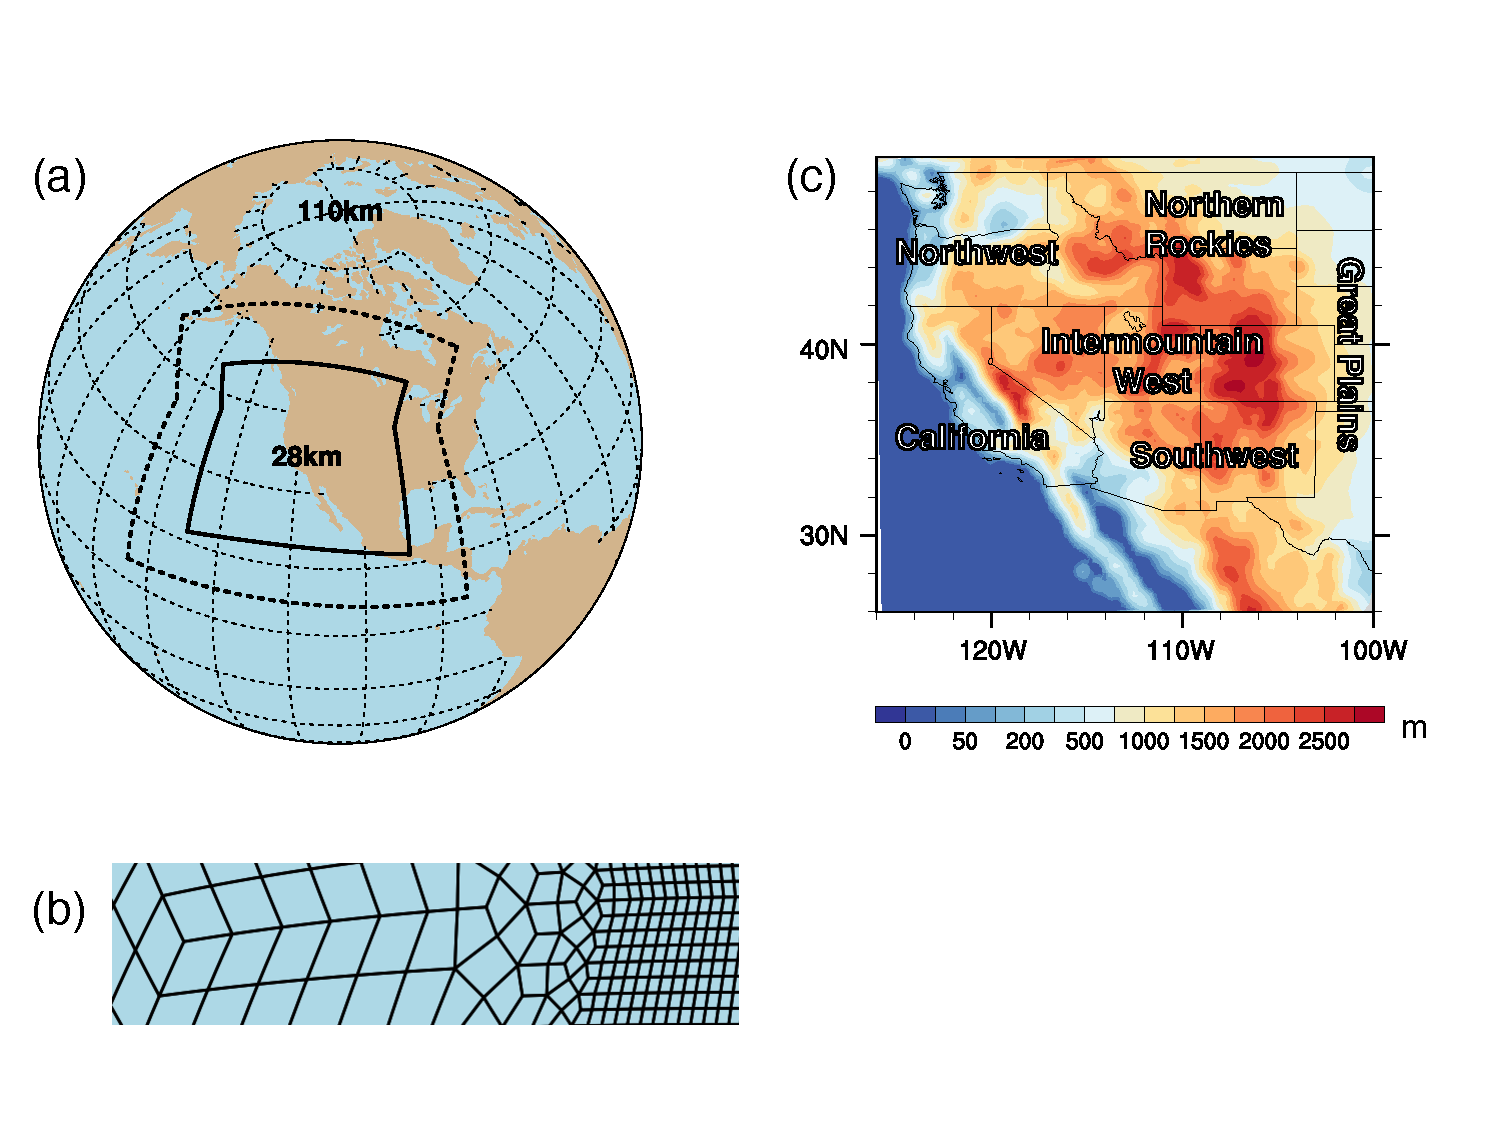
\includegraphics[width=5in]{gridmesh_mod.pdf}
\caption{(a) The approximate grid spacing used for the VR-CESM 0.25$^\circ$ mesh. (b) A depiction of the transition from the global $1^\circ$ resolution mesh through two layers of refinement to $0.25^\circ$. (c) Topography height over the study area.}
\label{fig:gridmesh}
\end{center}
\end{figure}  


%Figure 2
\begin{figure}
\begin{center}
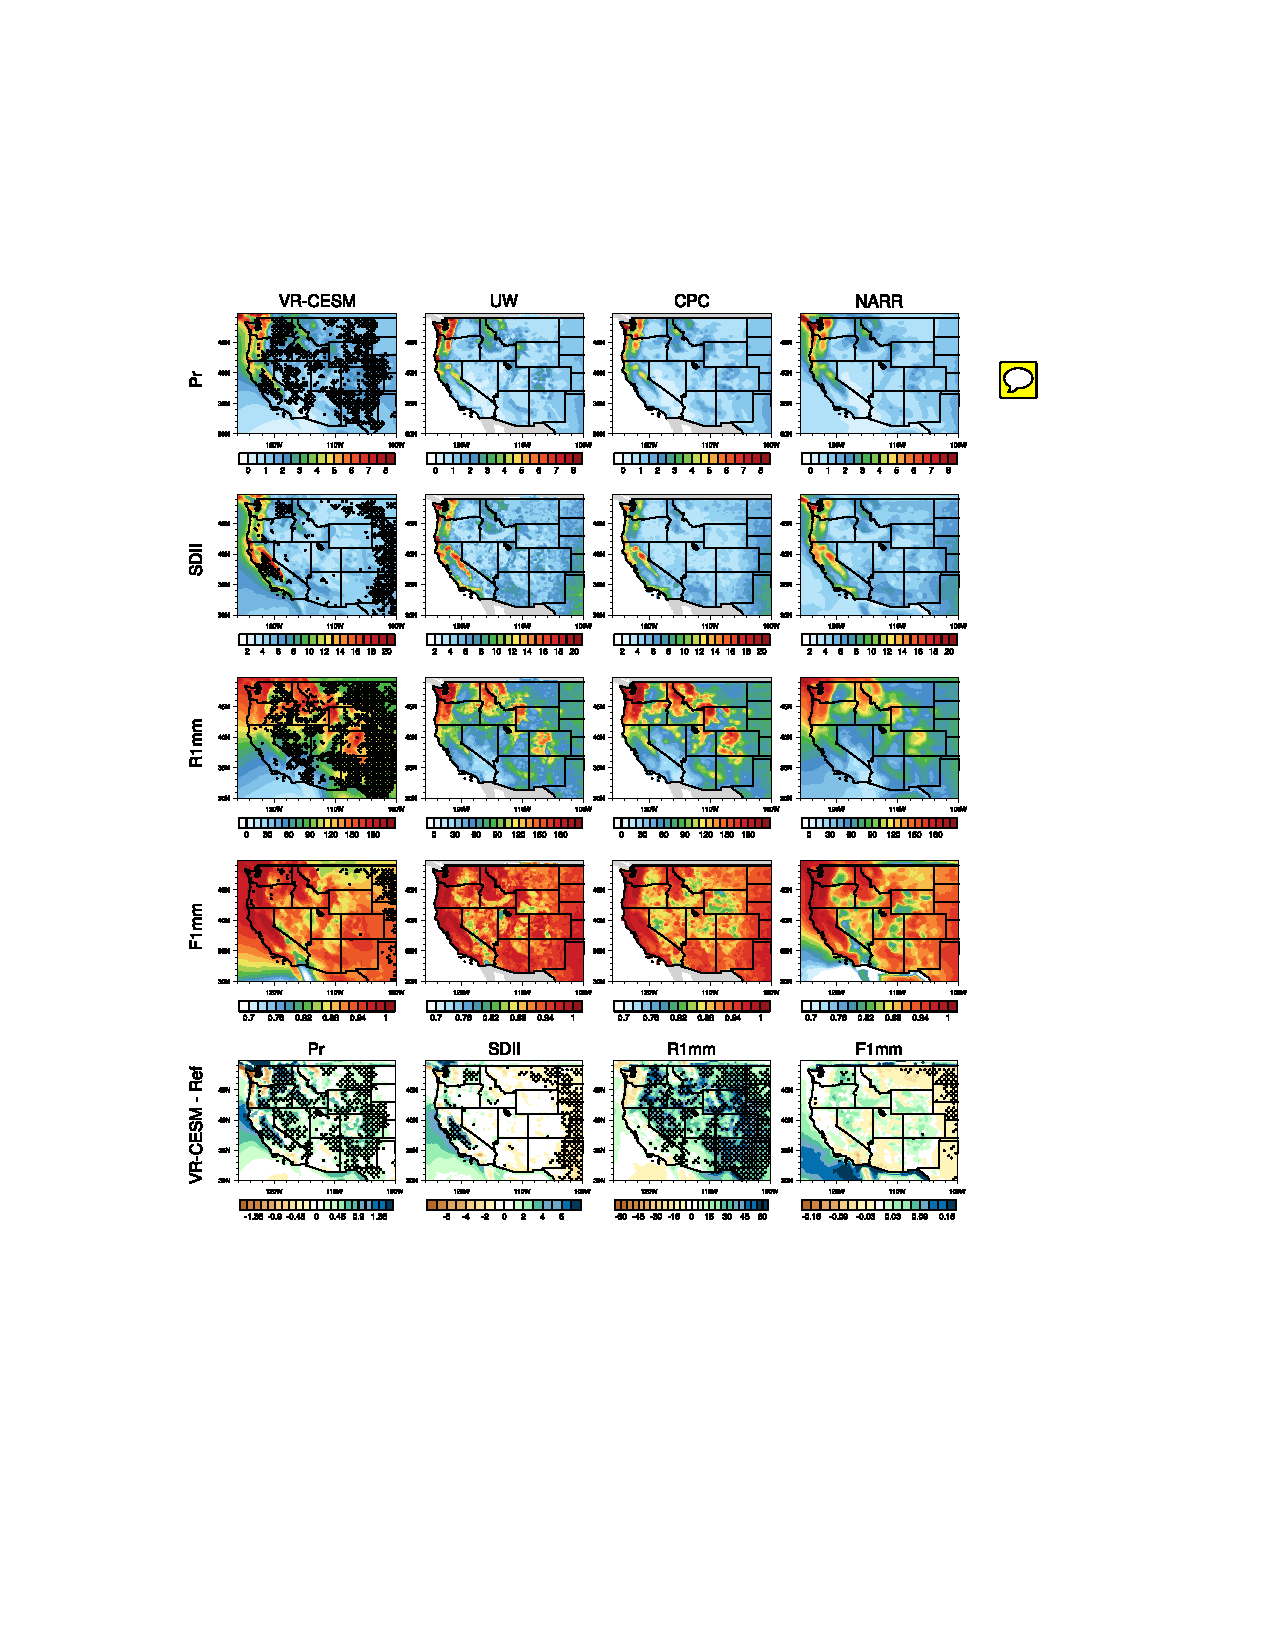
\includegraphics[width=6in, trim={3cm 6.5cm 5.2cm 4.9cm},clip]{wd_index_Hist_ref_annual_part1.pdf}
\caption{Mean precipitation and associated indices from VR-CESM and reference datasets over the historical period, 1980-2005.  Areas with statistically significance differences are marked with stippling.}
\label{fig:histEval1}
\end{center}
\end{figure}

%Figure 3
\begin{figure}
\begin{center}
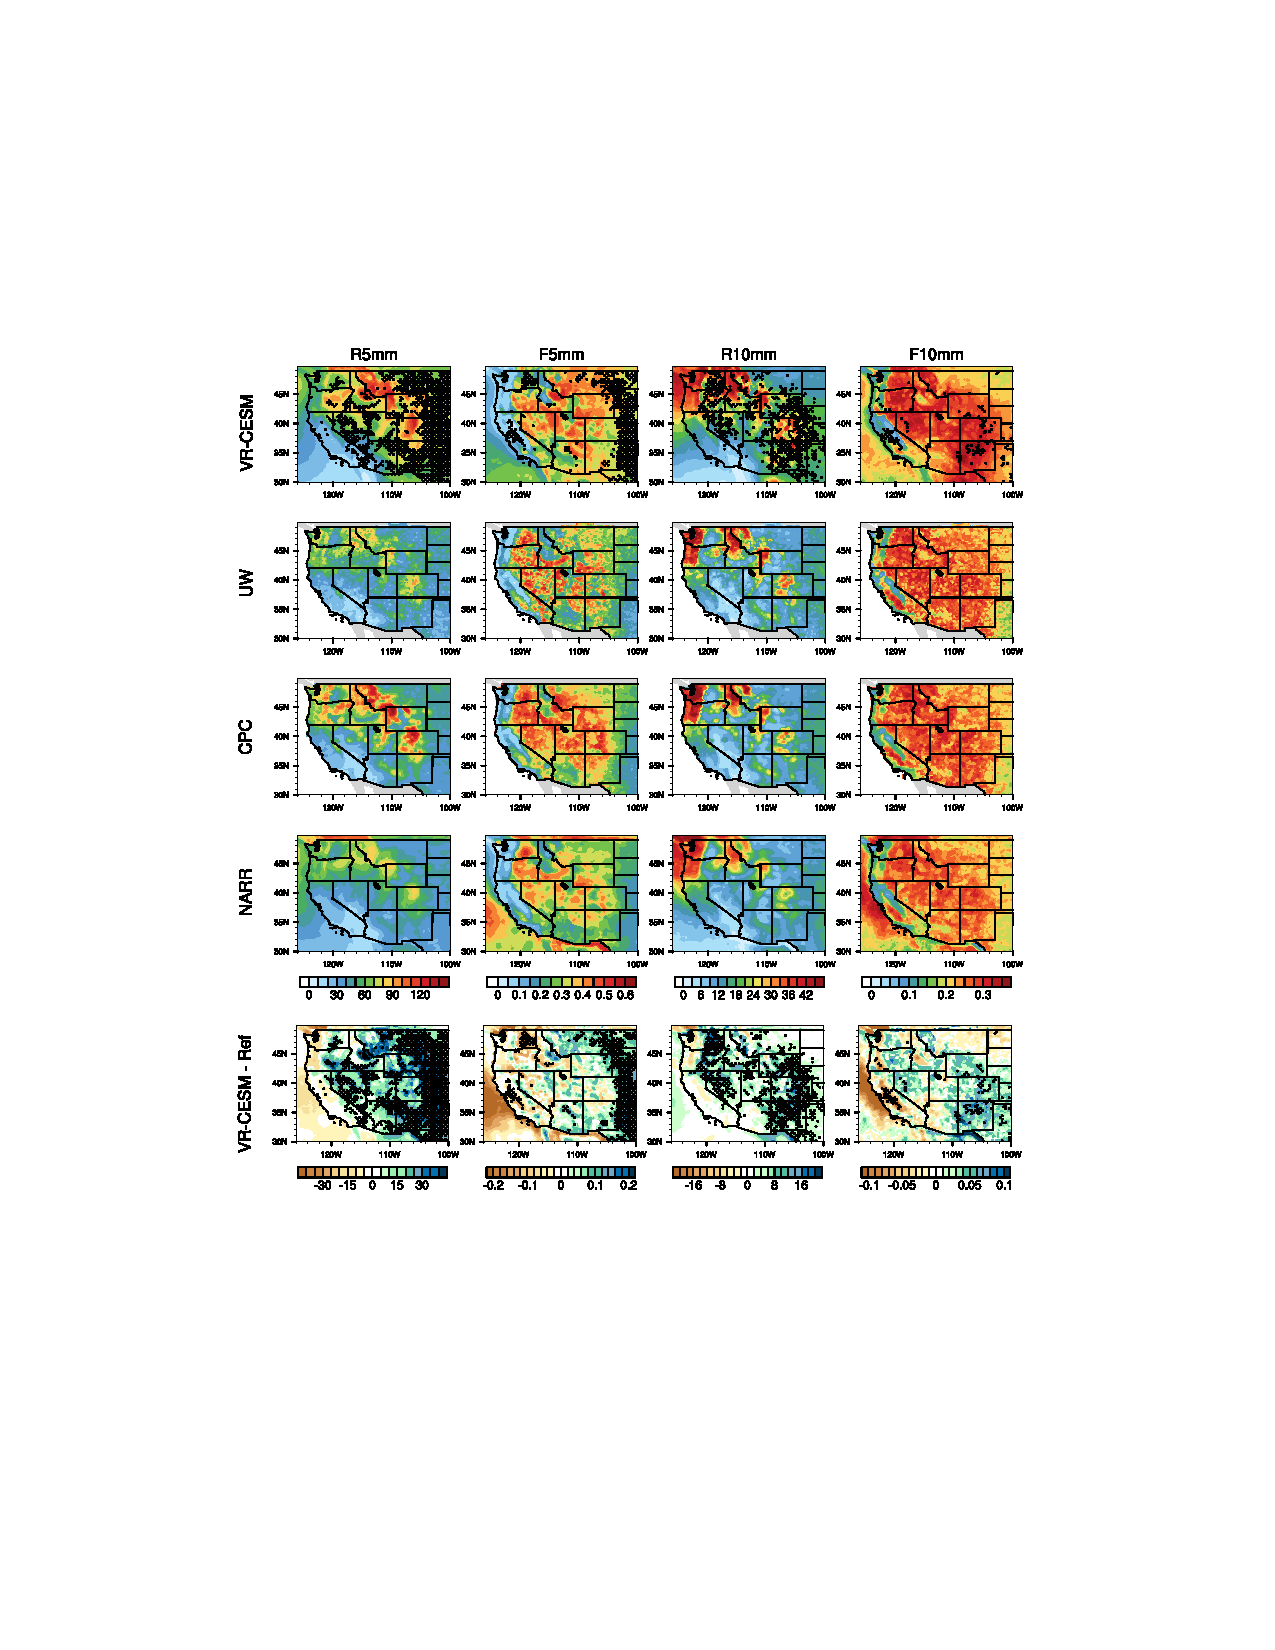
\includegraphics[width=6in, trim={4cm 6.5cm 4cm 4.9cm},clip]{wd_index_Hist_ref_annual_part2.pdf}
\caption{Mean precipitation and associated indices from VR-CESM and reference datasets over the historical period, 1980-2005 (continued).}
\label{fig:histEval2}
\end{center}
\end{figure}

%Figure 4
\begin{figure}
\begin{center}
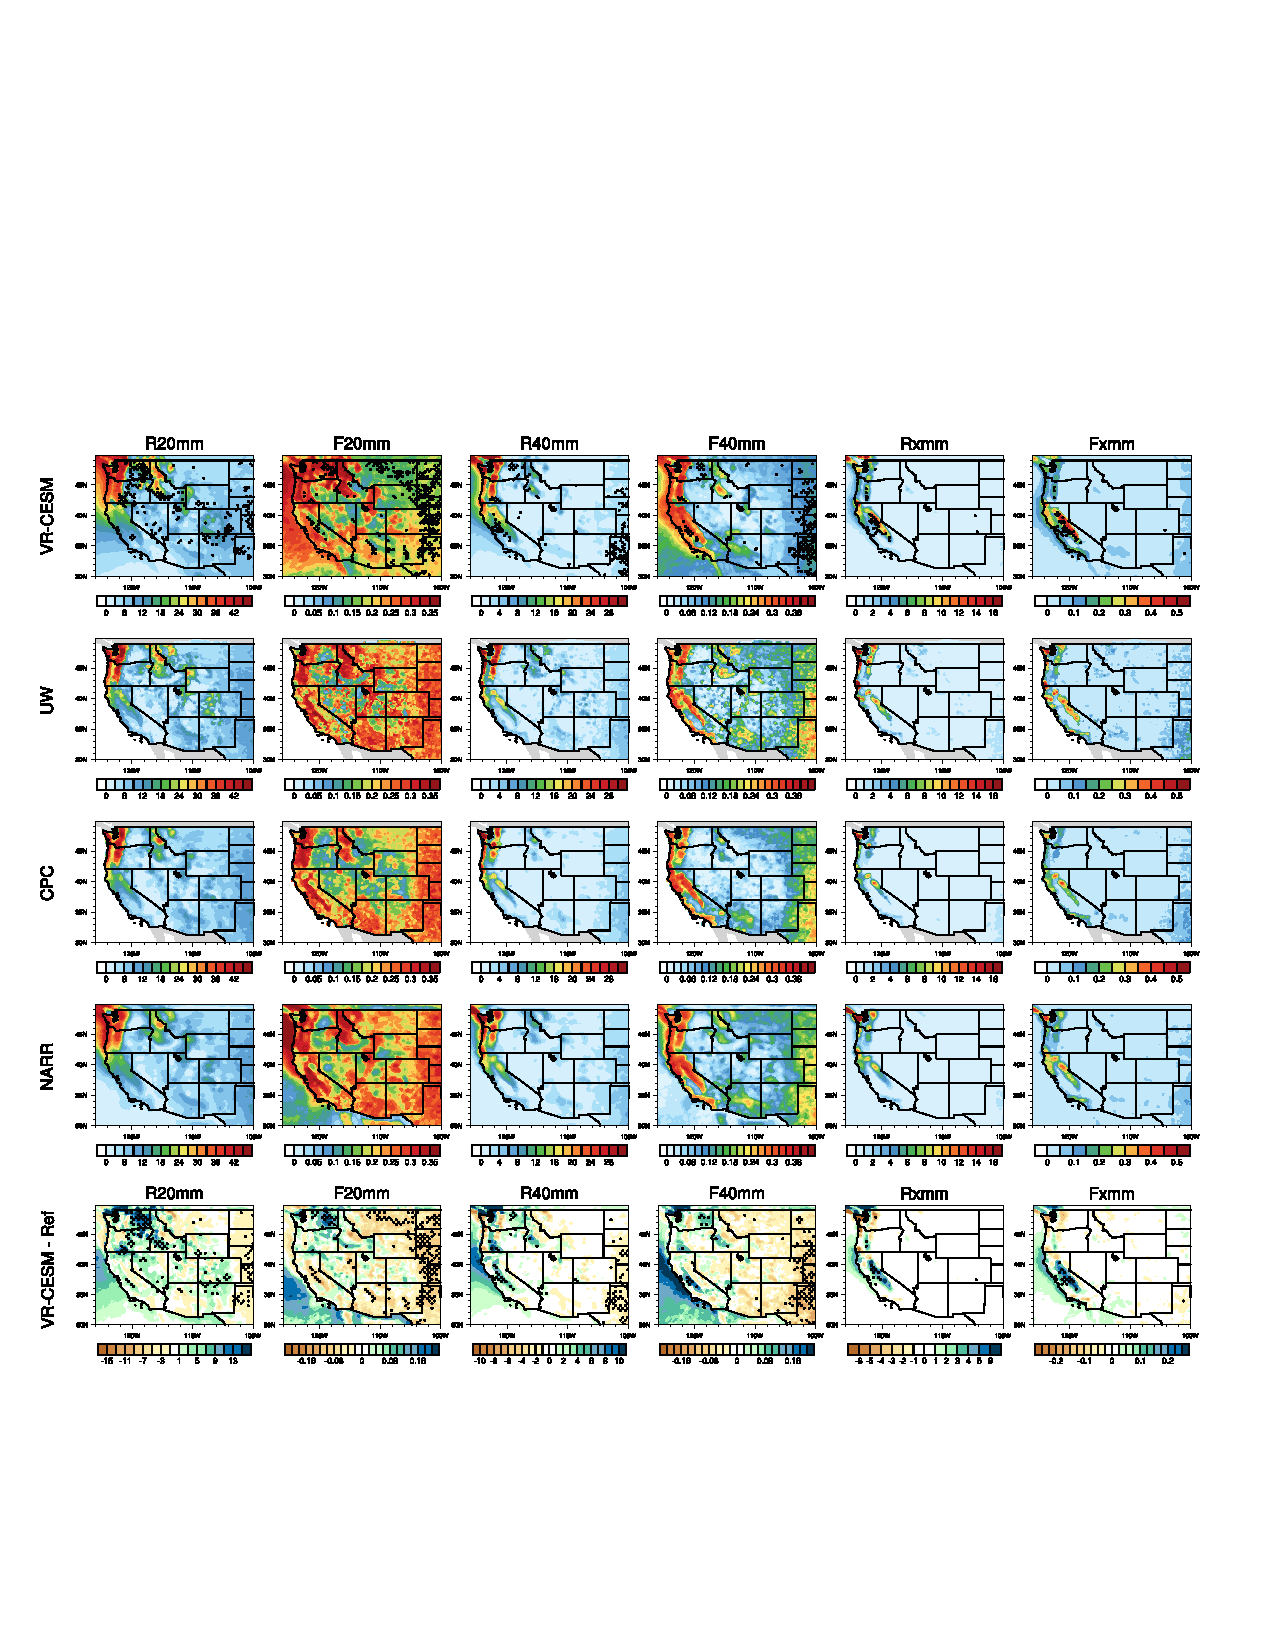
\includegraphics[width=6in, trim={0.6cm 4.5cm 1.2cm 4.9cm},clip]{wd_index_Hist_ref_annual_part3.pdf}
\caption{Mean precipitation and associated indices from VR-CESM and reference datasets over the historical period, 1980-2005 (continued).}
\label{fig:histEval3}
\end{center}
\end{figure}

%Figure 5
\begin{figure}
\begin{center}
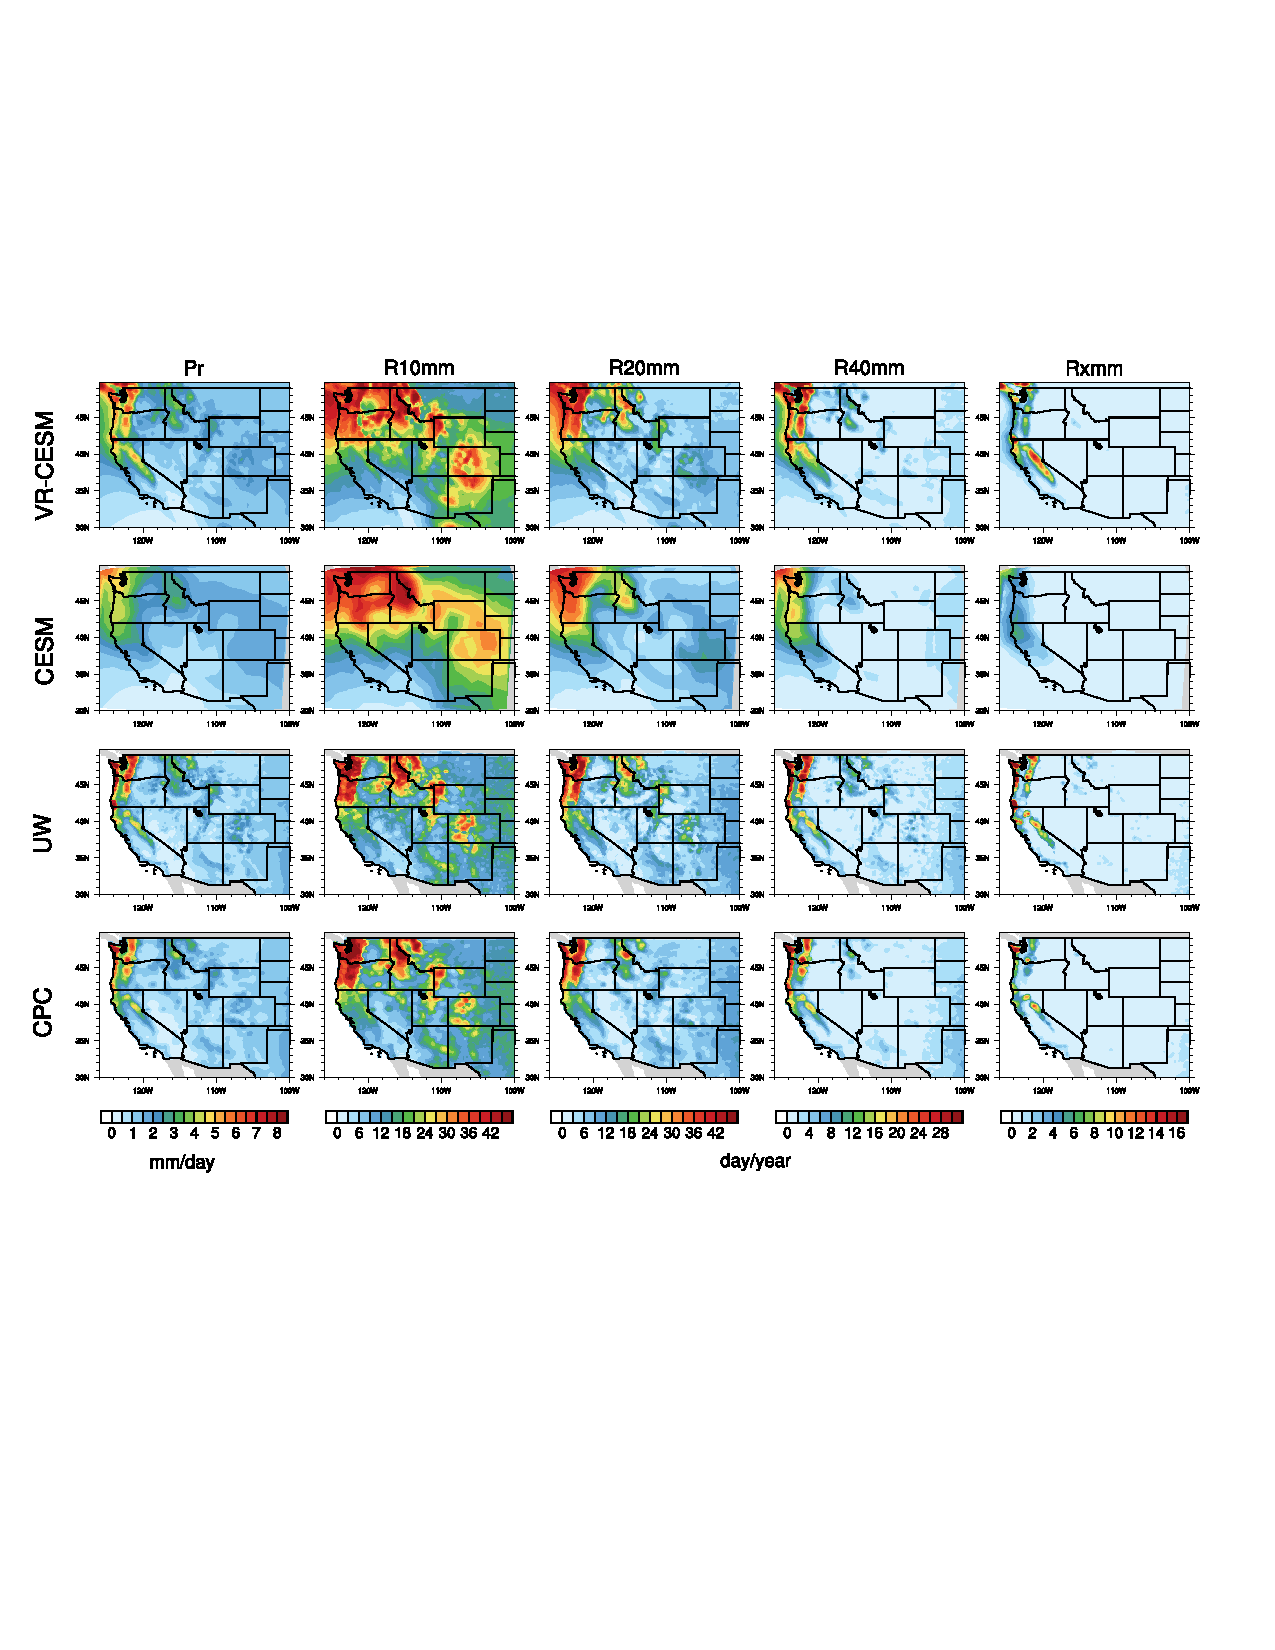
\includegraphics[width=6in]{wd_index_hist_vr_vs_1deg_cesm.pdf}
\caption{Mean precipitation and associated indices from VR-CESM and CESM at the resolution of 1$^\circ$ over the historical period, 1980-2005. Reference datasets (UW and CPC) are also included for better interpretation.}
\end{center}
\label{fig:resEffect}
\end{figure}


%Figure 6
\begin{sidewaysfigure}
\begin{center}
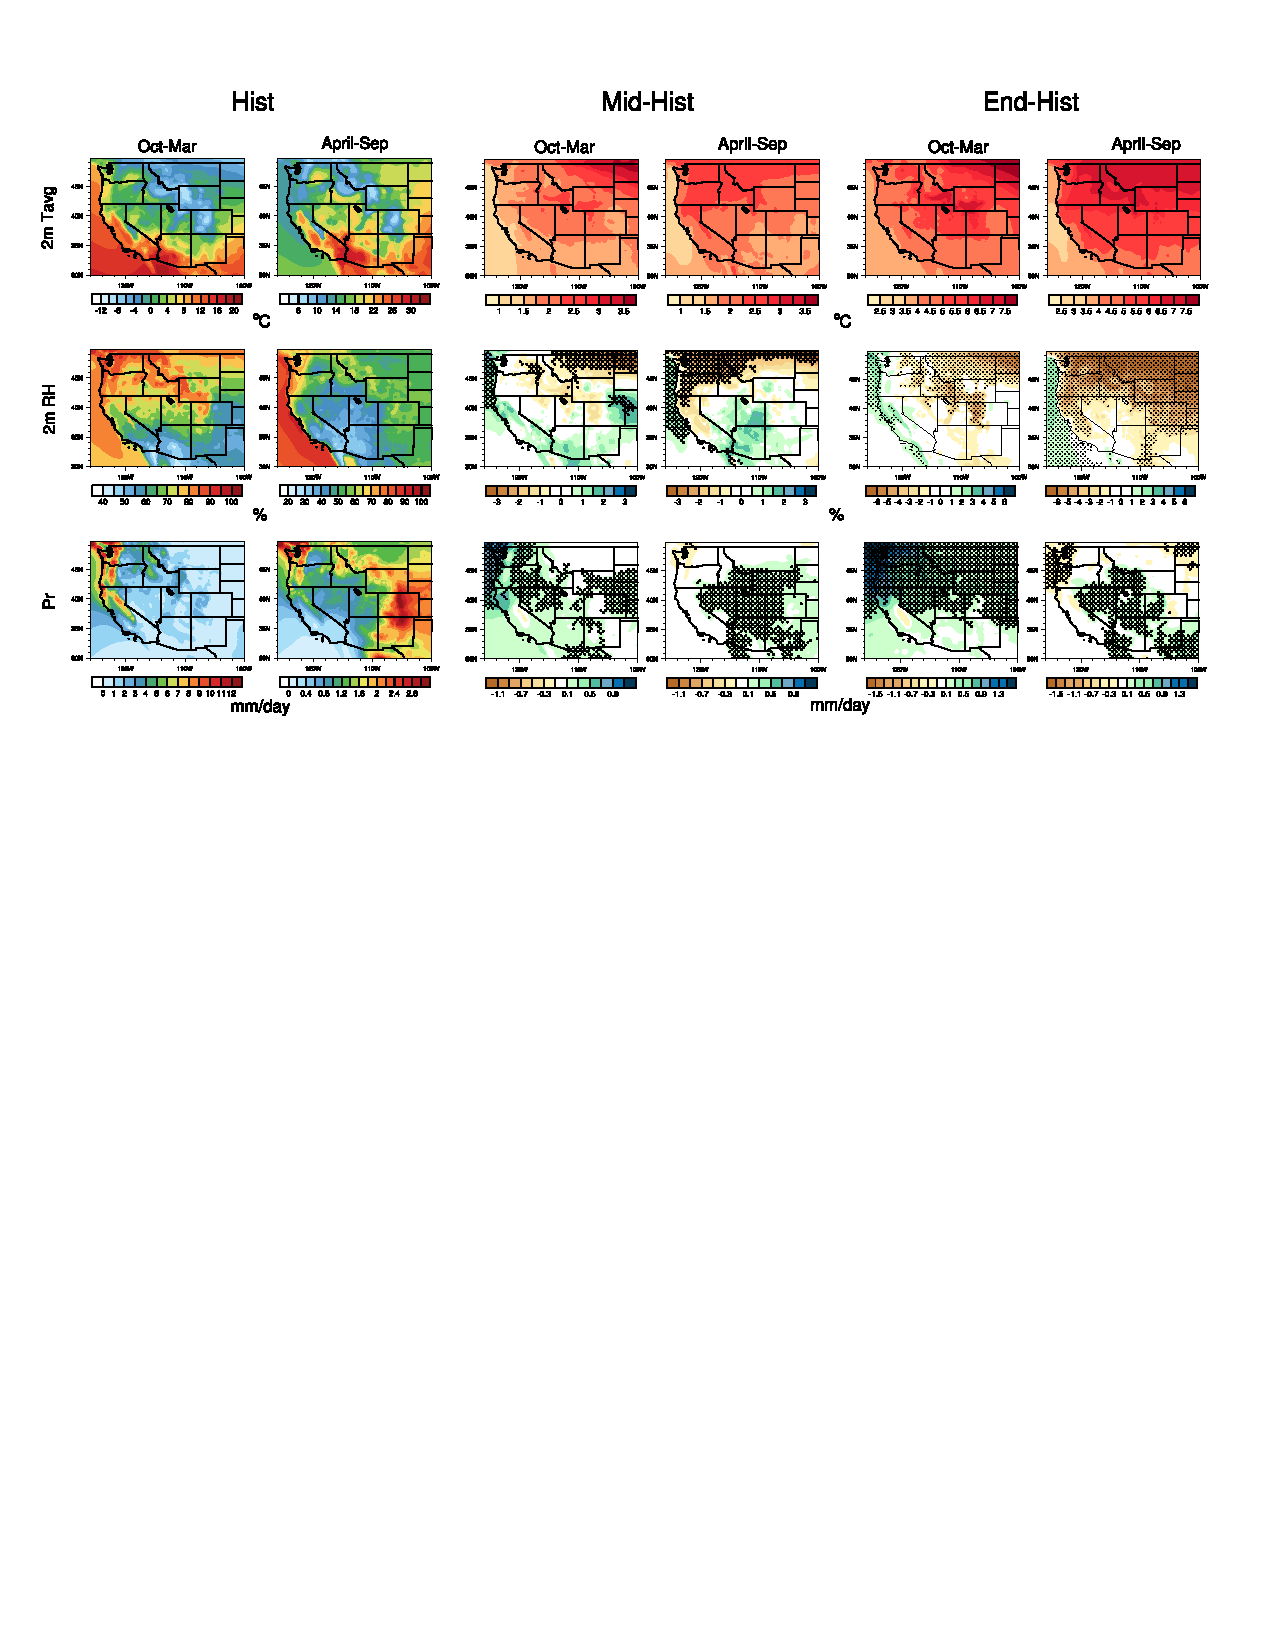
\includegraphics[width=8in, trim={0.6cm 15.5cm 1.0cm 1.0cm},clip]{pr_mean_clm.pdf}
\caption{2m average temperature (Tavg), 2m relative humidity (RH) and mean precipitation (Pr) averaged over the historical time period, along with average differences \textsf{mid}-\textsf{hist} and \textsf{end}-\textsf{hist}.  Areas with statistically significance differences are marked with stippling.}
\label{fig:meanClm}
\end{center}
\end{sidewaysfigure}

%Figure 7
\begin{figure}
\begin{center}
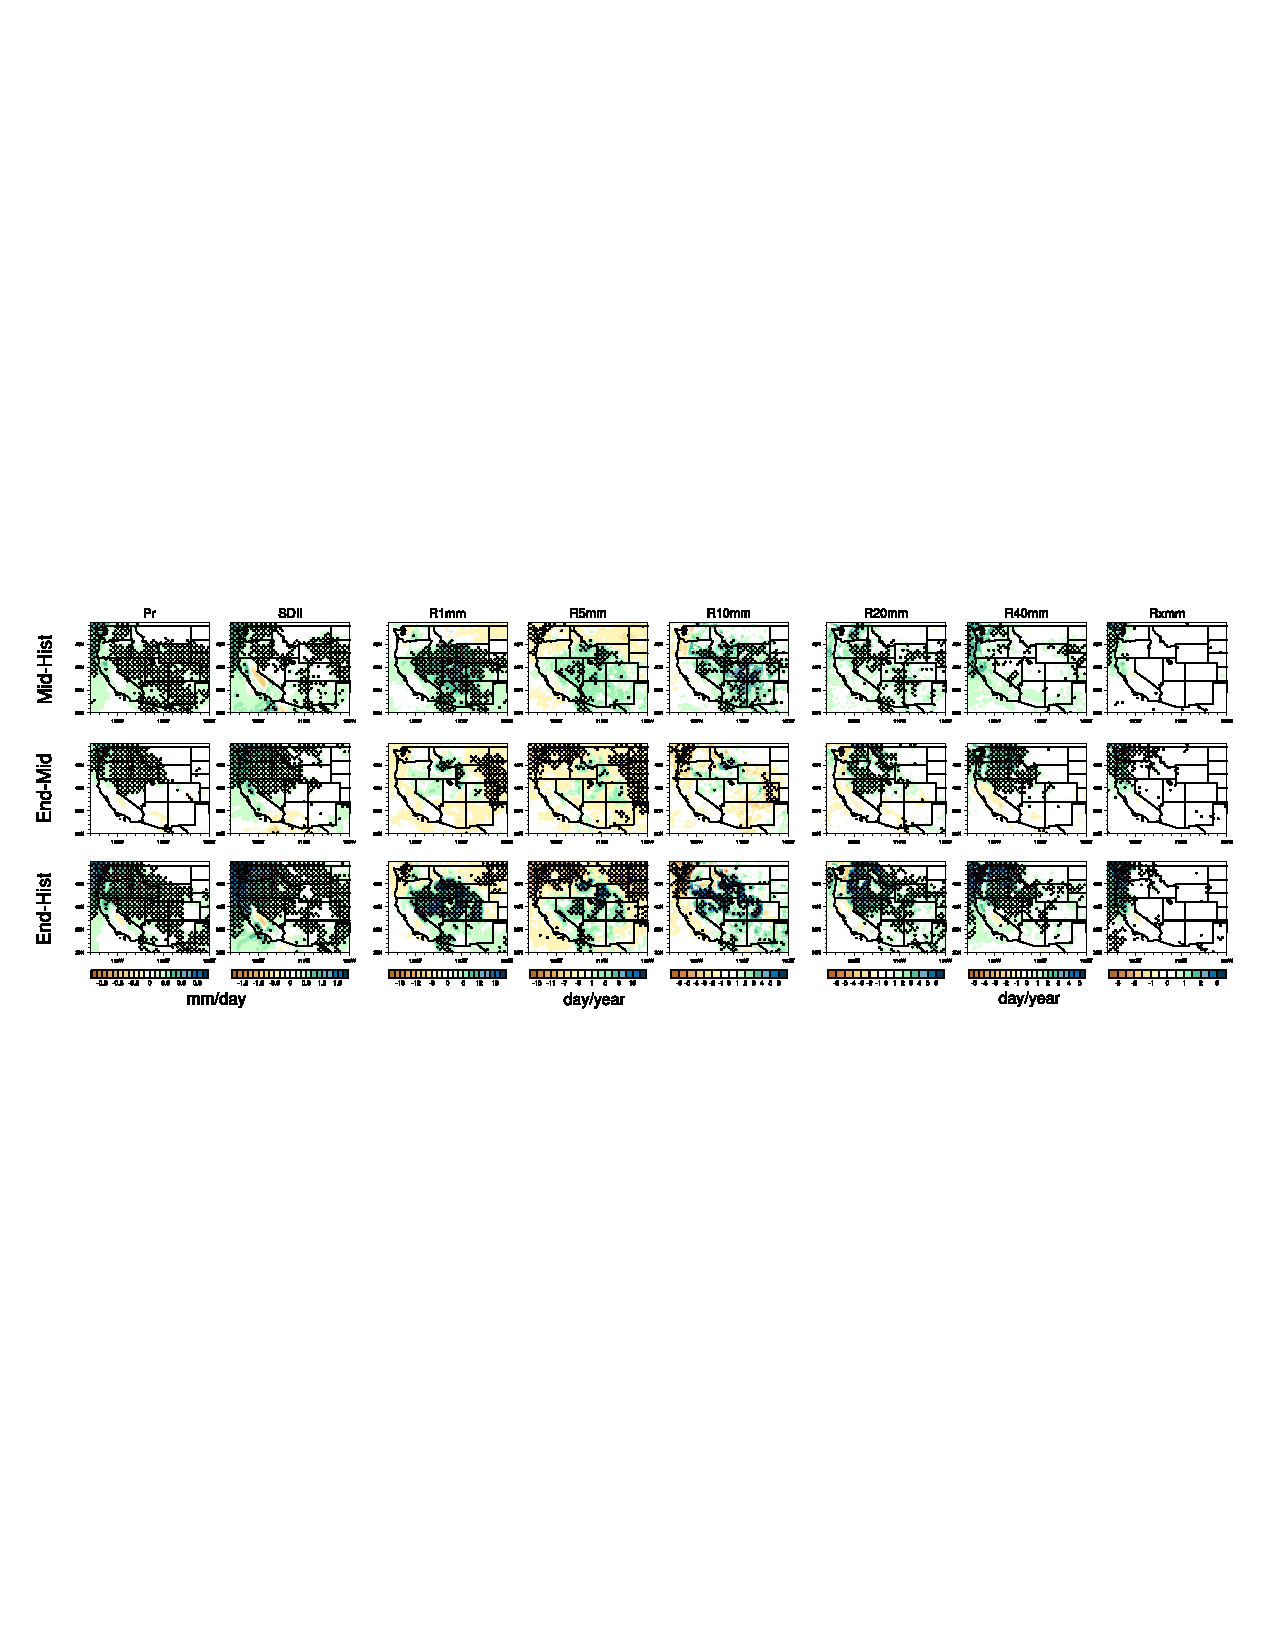
\includegraphics[width=6in, trim={3.5cm 6.5cm 3.5cm 2.0cm},clip]{wd_index_all_years_part1.pdf} %, angle = 90
\caption{Differences of precipitation indices Pr (mm/day), SDII and R$\ast$mm between \textsf{hist}, \textsf{mid} and \textsf{end} average.  Areas with statistically significance differences are marked with stippling.}
\label{fig:difIndex1}
\end{center}
\end{figure}


%Figure 8
\begin{sidewaysfigure}
\begin{center}
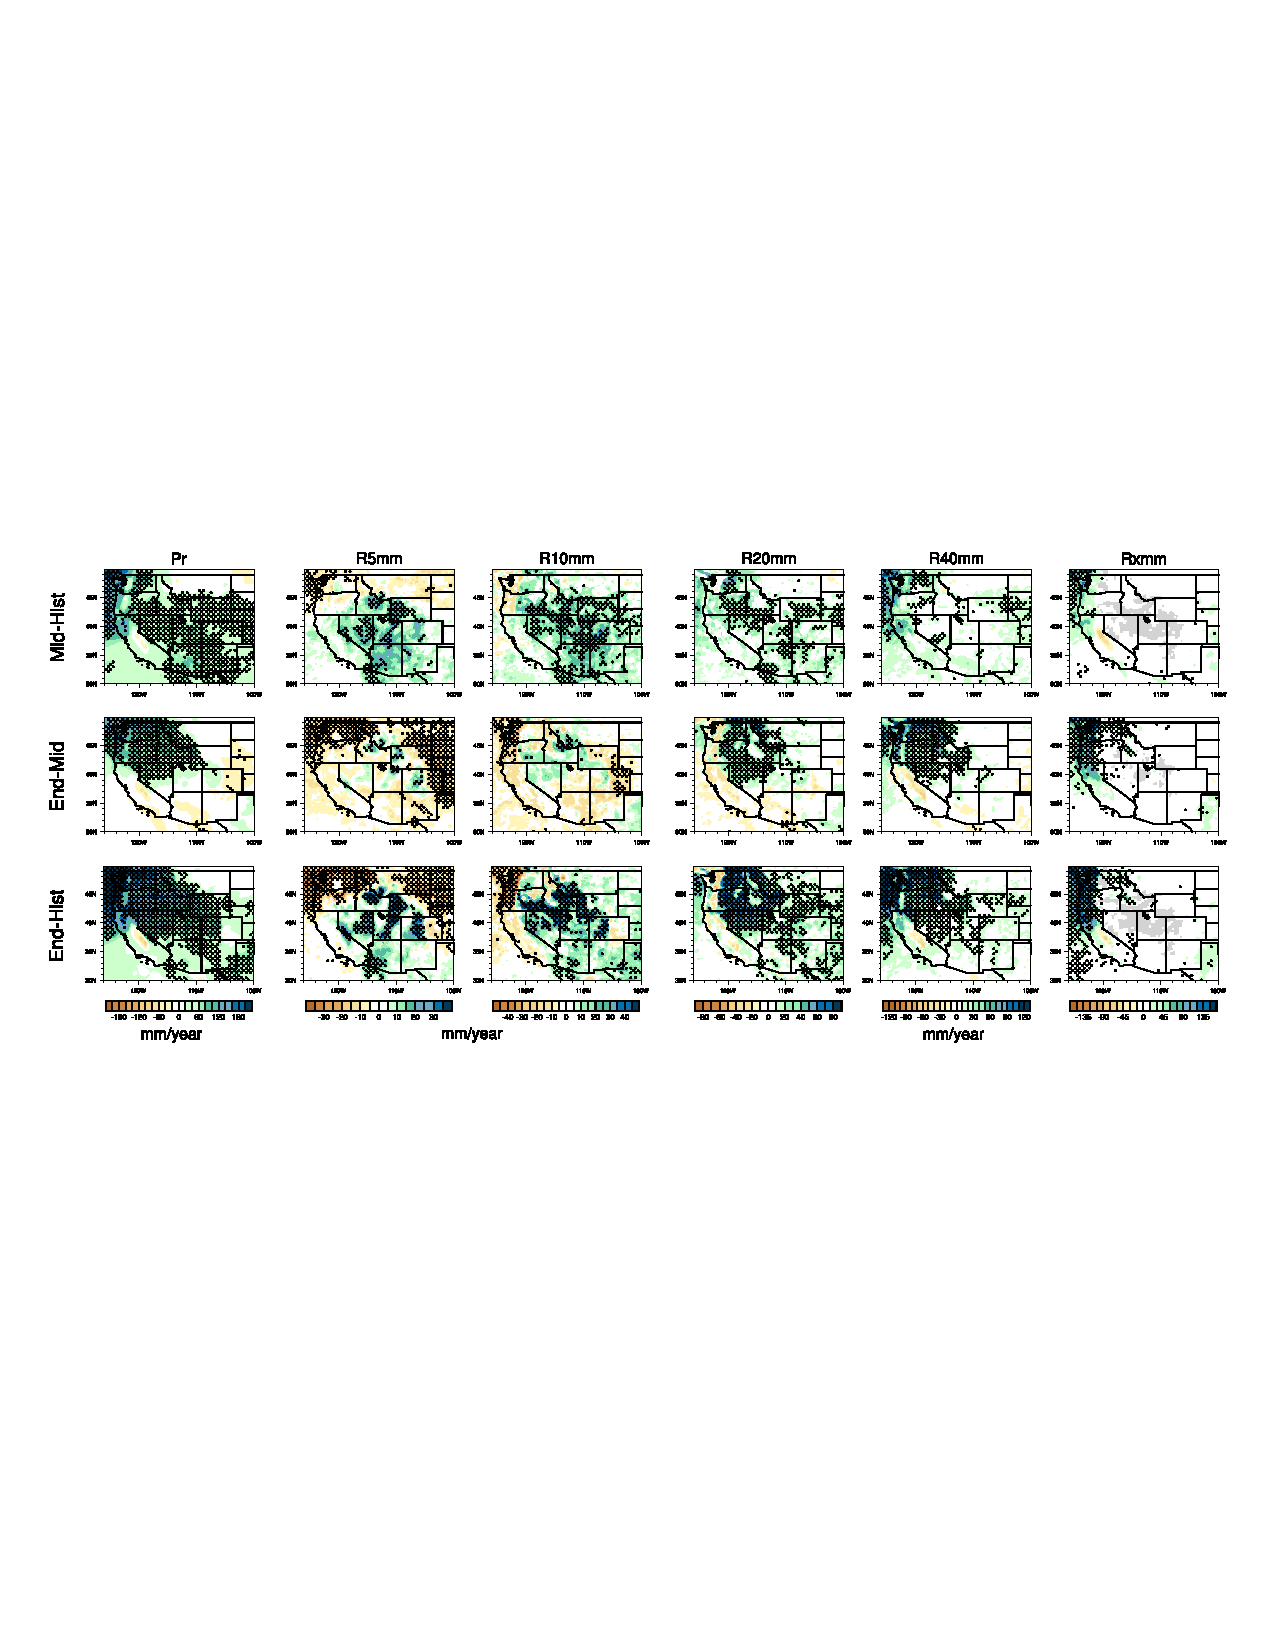
\includegraphics[width=8in, trim={0.6cm 9.5cm 1.0cm 9.0cm},clip]{wd_index_all_years_part2.pdf}
\caption{Differences of precipitation indices Pr (mm/year) and P$\ast$mm between \textsf{hist}, \textsf{mid} and \textsf{end} average.  Areas with statistically significance differences are marked with stippling.  Areas with no data are indicated in gray.}
\label{fig:difIndex2}
\end{center}
\end{sidewaysfigure}

%Figure 9
\begin{figure}
\begin{center}
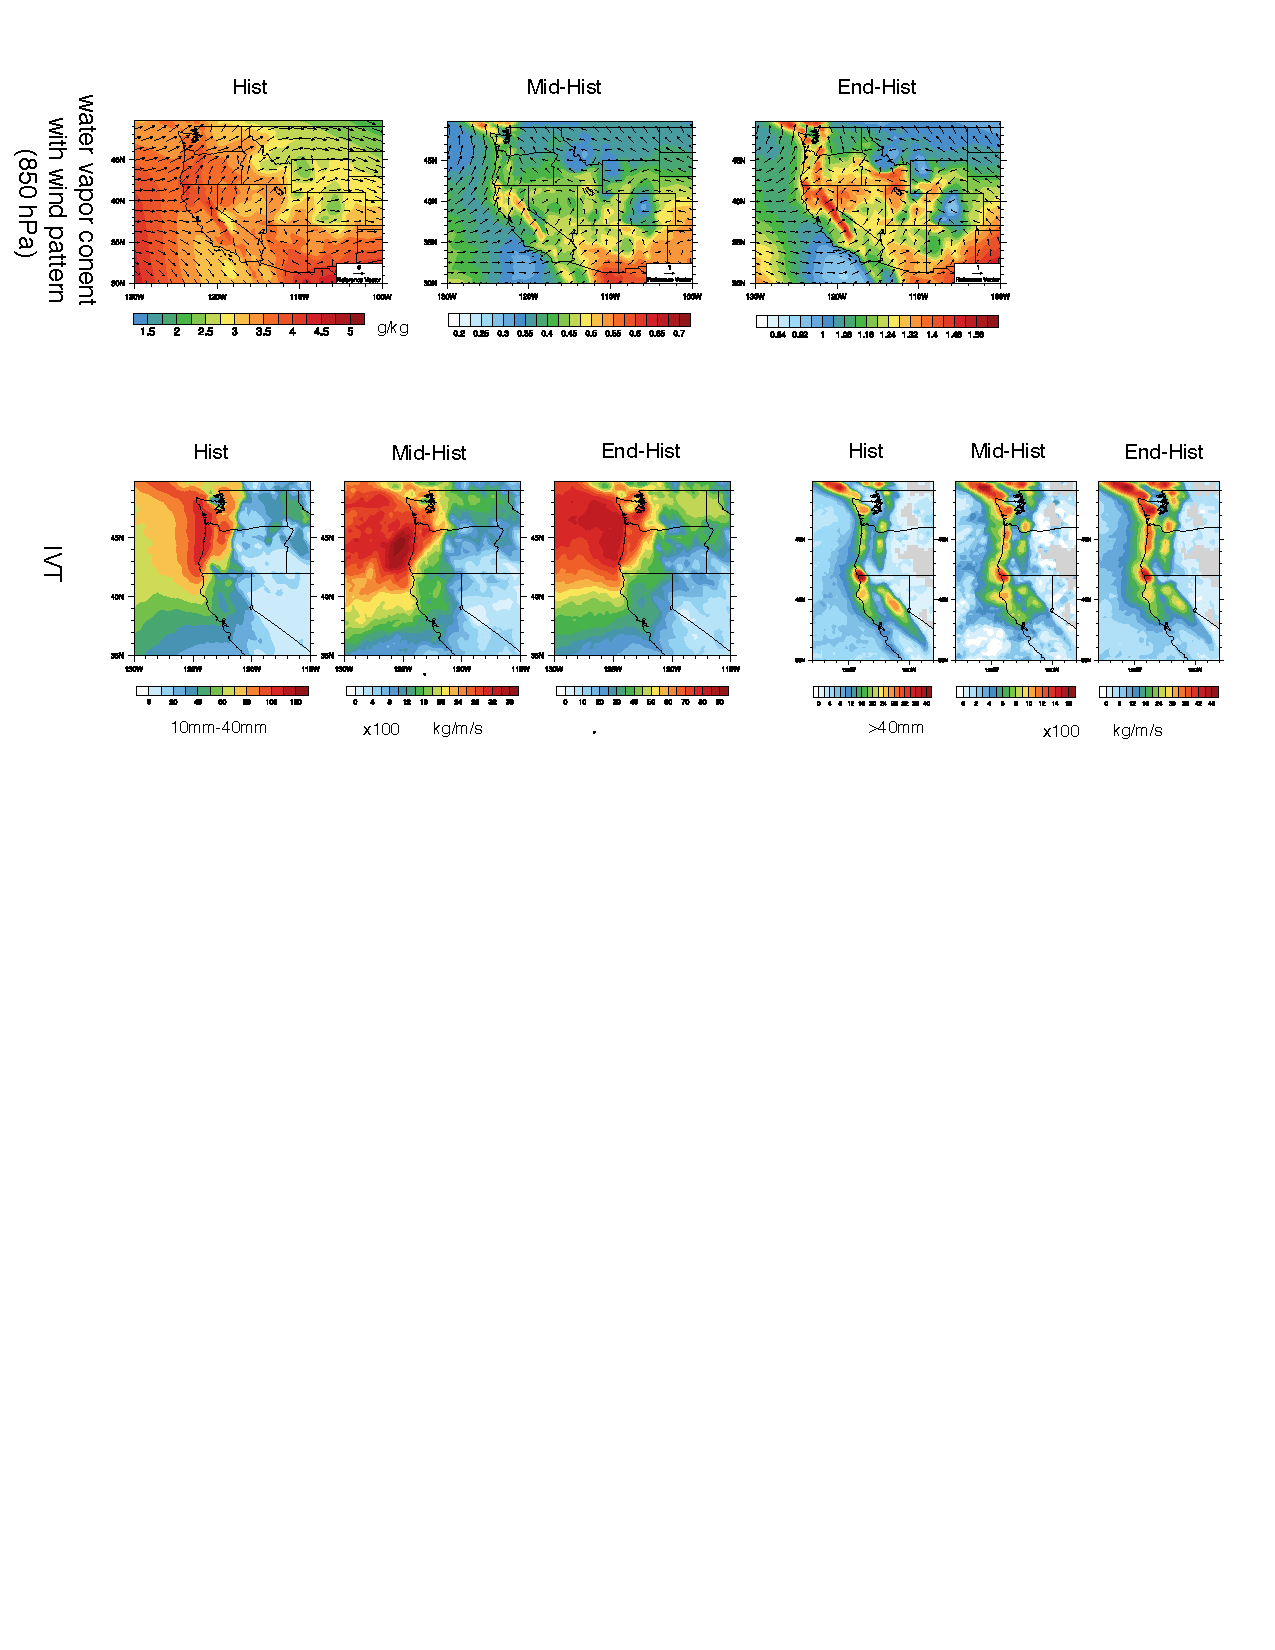
\includegraphics[width=6in]{discussion_indices.pdf}
\caption{Differences in specific humidity and horizontal wind patterns at 850hPa for moisture flux, and pointwise IVT (averaged over days with (a) 10mm$<$Pr$<=$40mm and (b) Pr$>$40mm) for the cool season (October to March) averaged over 26 years. The minimum wind vector length is set to 0.5 m/s for better visualization. (Lower plot) Specific humidity and wind patterns are averaged over all days over cool season.}
\label{fig:discussIndex}
\end{center}
\end{figure}

%Figure 10
\begin{figure}
\begin{center}
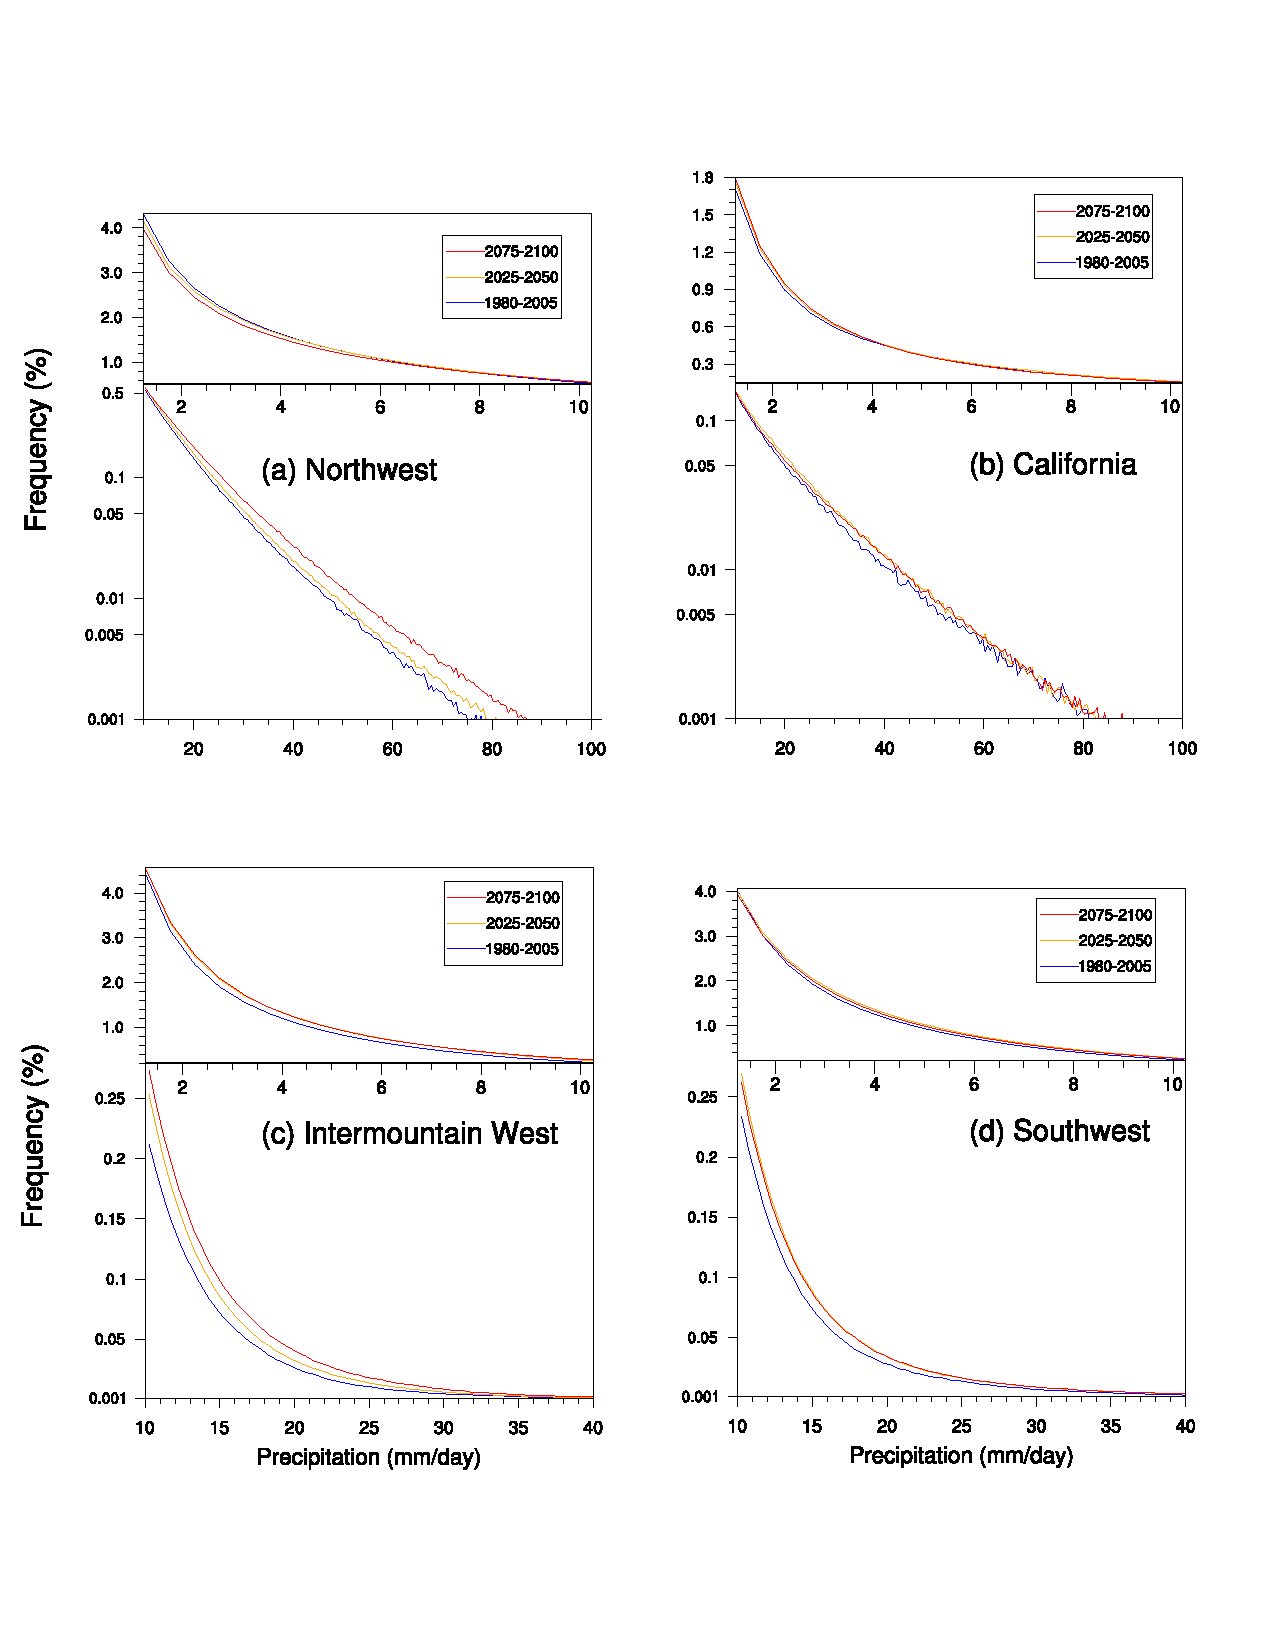
\includegraphics[width=6in]{PP_PDF_region1_4.pdf}
\caption{Frequency distribution of rainy days (Pr$>=$0.1mm$/$day) over the three time periods from all simulations dataset in four regions (with logarithmic vertical scale). (Note: Region (a) to (d) cover Washington and Oregon; California (except northern part, i.e. latitude no larger than 38$^\circ$); Nevada and Utah; Arizona and New Mexico, respectively.)}
\label{fig:prPDF}
\end{center}
\end{figure}

%Figure 11
\begin{figure}
\begin{center}
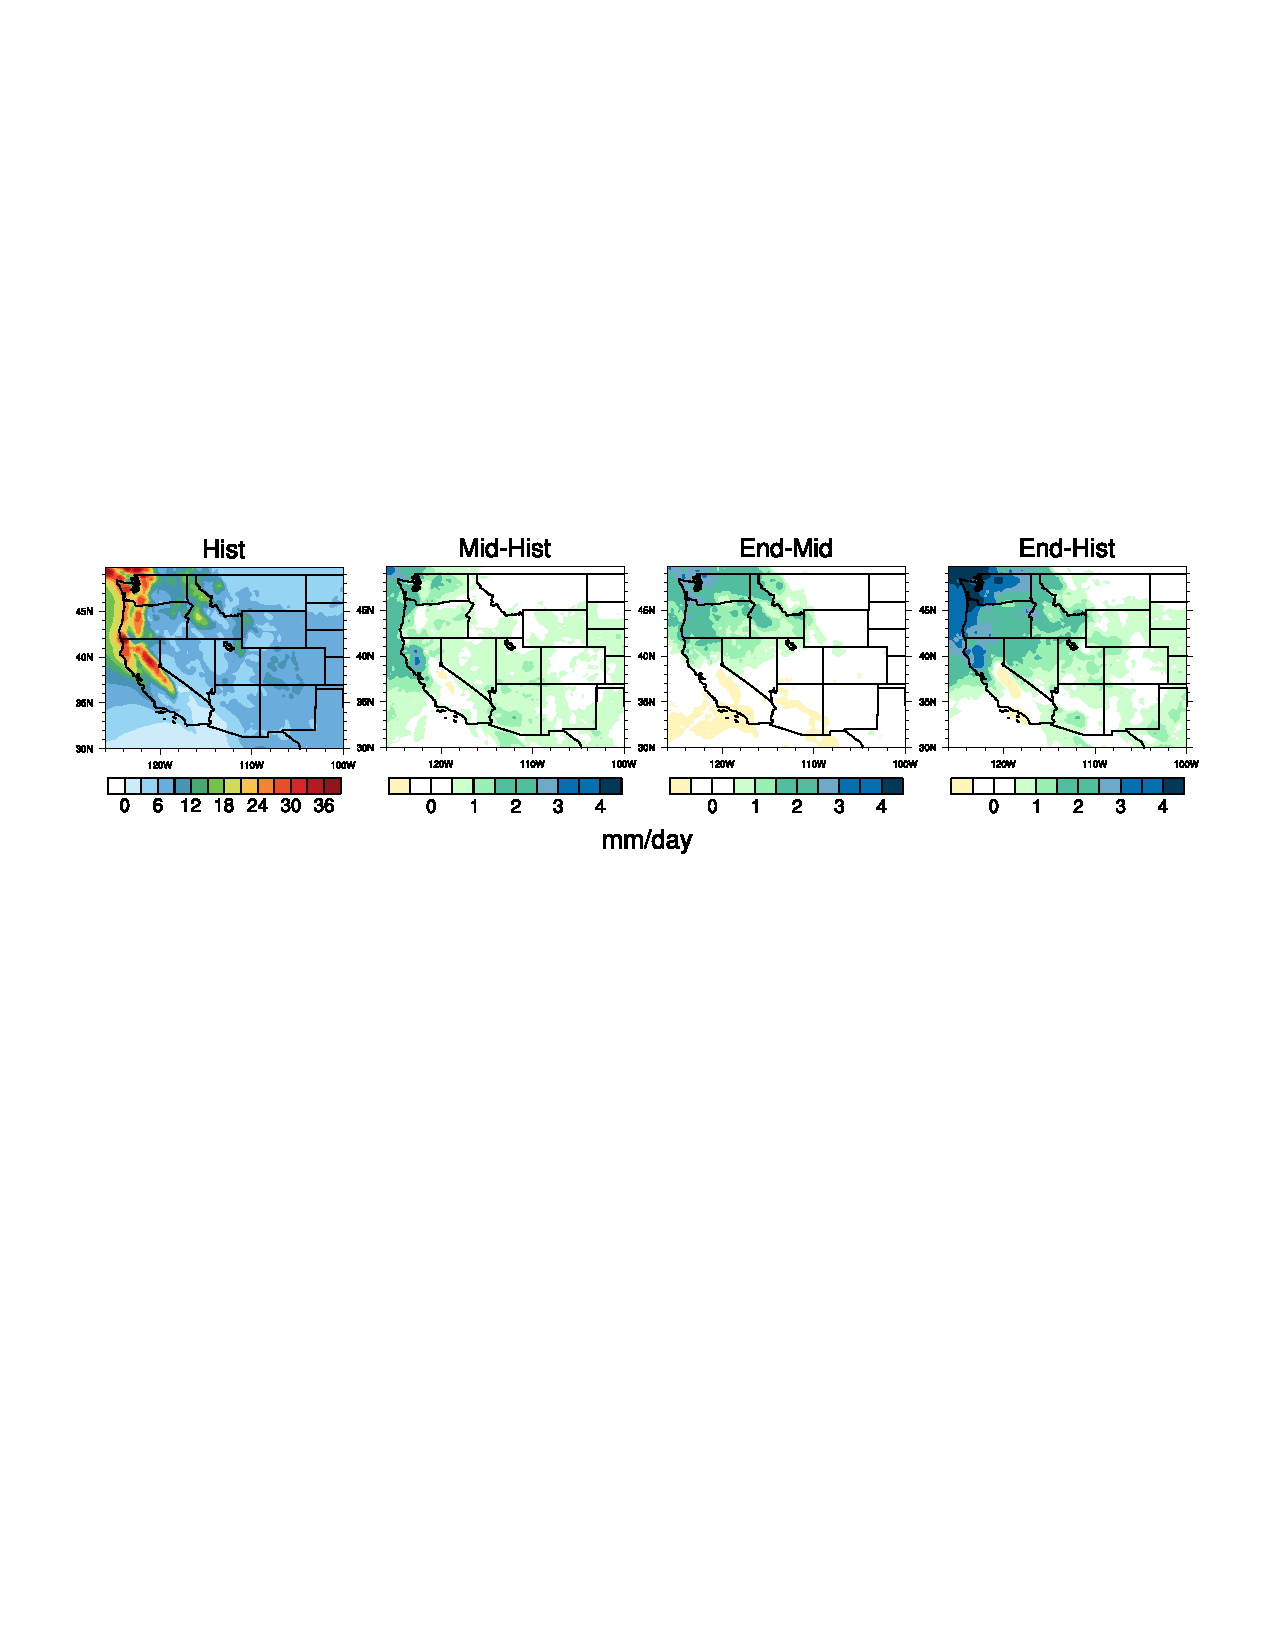
\includegraphics[width=6in]{extreme_percentile.pdf}
\caption{The 95th percentile (P95) of precipitation constructed from all days for the historical period, 1980-2005 and the changes over each future time period.}
\label{fig:prQtile}
\end{center}
\end{figure}

%Figure 12
\begin{sidewaysfigure}
\begin{center}
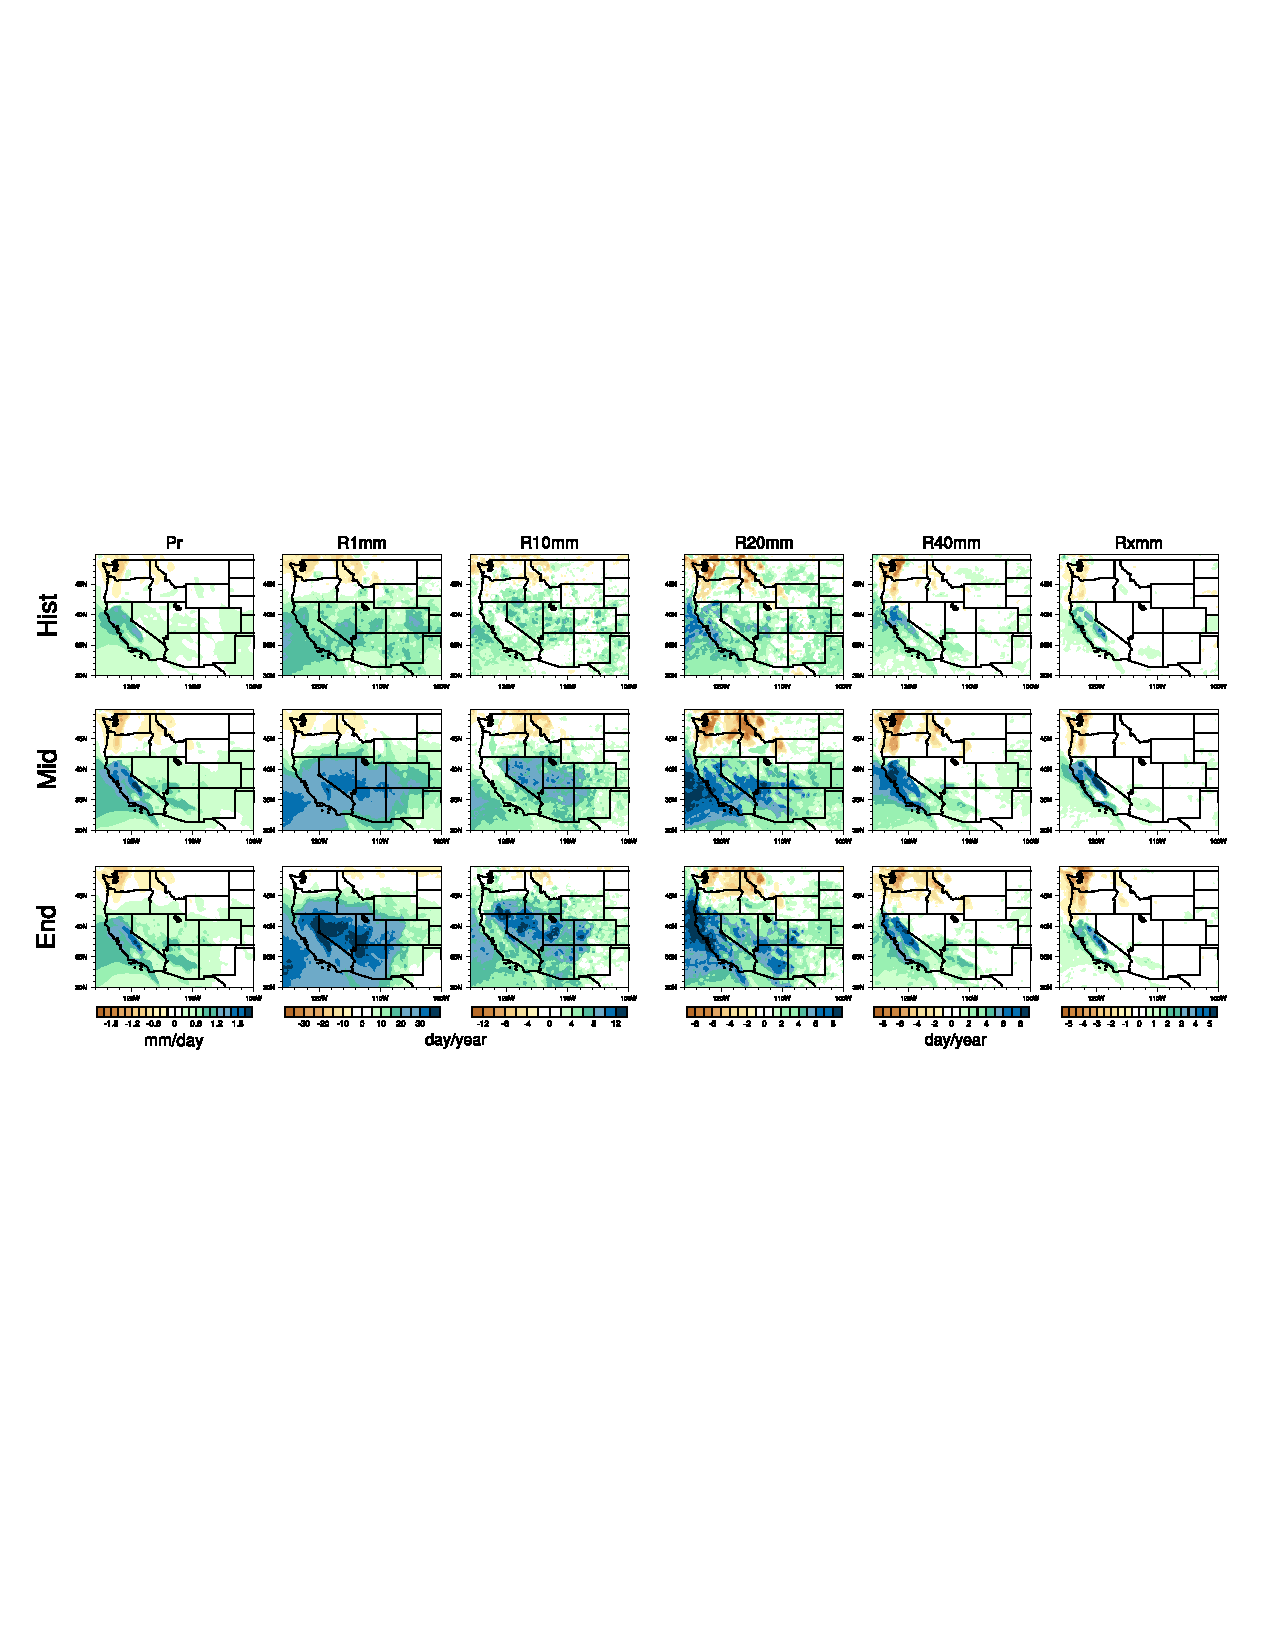
\includegraphics[width=8in, trim={0.6cm 9.5cm 1.0cm 9.0cm},clip]{wd_index_enso_wetSeason.pdf}
\caption{Differences of precipitation indices Pr and R$\ast$mm between warm and cool phases of ENSO over each time period.}
\label{fig:difEnso}
\end{center}
\end{sidewaysfigure}

%Figure 13
\begin{figure}
\begin{center}
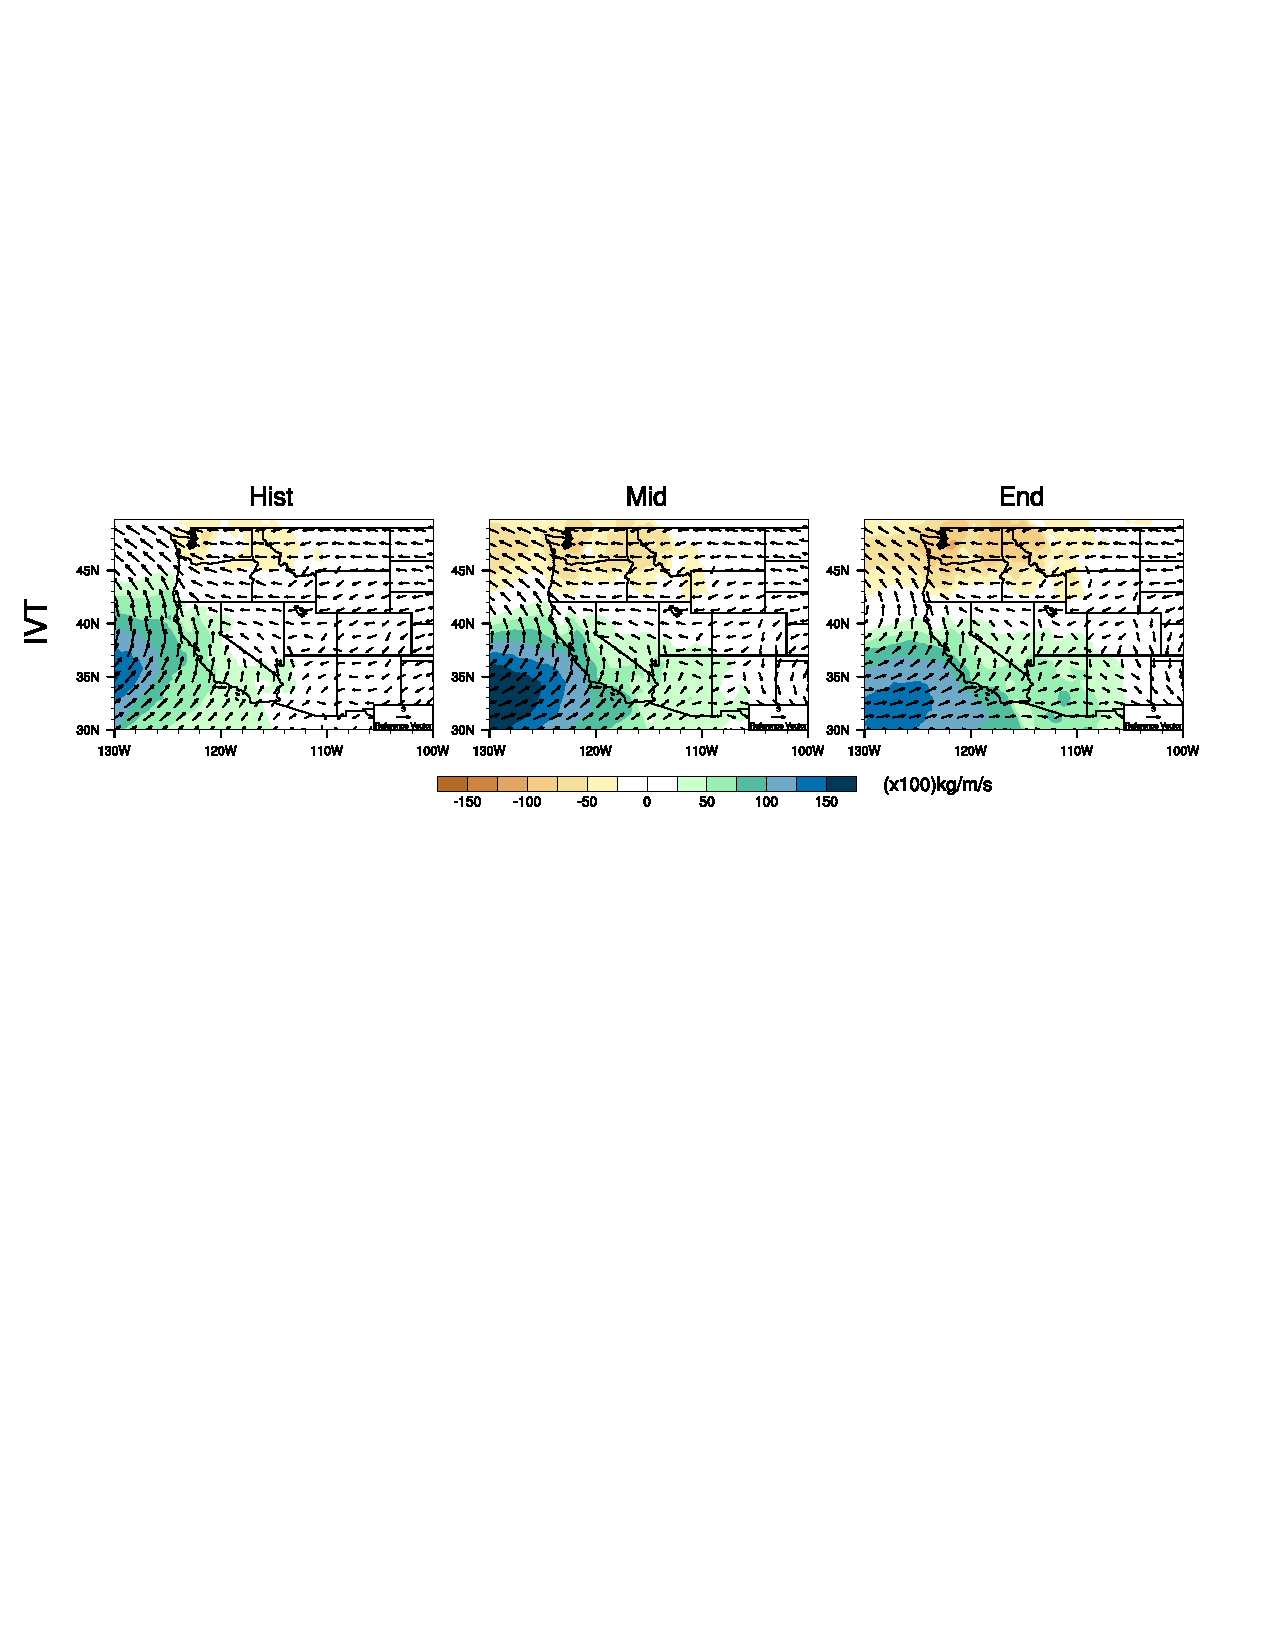
\includegraphics[width=6in]{discussion_enso.pdf}
\caption{Changes of IVT for simulations under different phases of ENSO of wet season (October to March) over rainy days averaged yearly, with seasonal mean wind patterns at 850hPa (unit: m/s) (Note: The minimum wind vector is set to be 0.5 m/s, therefore, the wind less than 0.5 m/s is also plotted at the minimum length for better visualization.)}
\label{fig:discussEnso}
\end{center}
\end{figure}

%%%%%%%%%%%%%%%%%%%%%%%%%%%


\end{document}
